\chapter{Уравнения первого порядка, разрешённые относительно производной}

\section{Основные понятися и результаты}

\subsection{Объект изучения}

Рассмотрим обыкновенное дифференциальное уравнение первого порядка, разрешённое относительно проиводной:
\begin{equ}{1.1}
    \frac{\di y(x)}{\di x}, \qquad \text{или в краткой записи } y' = f(x, y)
\end{equ}

где $ x $ -- это независимая переменная, $ y = y(x) $ -- искомая функция, а $ f(x, y) $, \nimp, -- вещественная функция, определённая и непрерывная на множестве $ \vawe{G} = G \cup \hat{G} $, где:
\begin{itemize}
	\item $ G \sub \R^2 $ -- область
    \item $ \hat{G} \subseteq \partial G $ -- (возможно пустое) множество, на котором $ f(x, y) $ непрерывна или может быть доопределена с сохранением непрерывности
\end{itemize}

\begin{remind}
	Область -- связное открытое множество
\end{remind}

\begin{notation}
    $ G^* \define \partial G \setminus \hat{G} $
\end{notation}

\subsection{Решения дифференциального уравнения}

\begin{notation}
	Символ $ \langle $ подразумевает одну из скобок: $ ( $ или $ [ $, а символ $ \rangle $ -- скобку $ ) $ или $ ] $
\end{notation}

На вещественной оси рассмотрим непустое связное множество, не являющееся точкой. Это будет промежуток $ \braket{a, b} $

\begin{definition}
    Функция $ y = \vphi(x) $, заданная на промежутке $ \braket{a, b} $ называется решением дифференциального уравнения \eref{1.1}, если для любого $ x \in \braket{a, b} $ выполняются следующие три условия:
    \begin{enumerate}
        \item функция $ \vphi(x) $ дифференцируема
        \item точка $ \big( x, \vphi(x) \big) \in \vawe{G} $
        \item $ \vphi'(x) = f\big( x, \vphi(x) \big) $
    \end{enumerate}
\end{definition}

\begin{remark}
	График решения по определению не может состоять из одной точки
\end{remark}

\begin{remark}
	Первые два условия являются вспомогательными и позволяют записать третье
\end{remark}

\begin{remark}
    Любое решение является функцией не просто дифференцируемой, а гладкой, т. е.
    $$ \vphi(x) \in \Cont[1]{\braket{a, b}} $$
\end{remark}

\begin{proof}
    Функция $ \vphi(x) $ дифференцируема (по условию 1). Значит, она непрерывна в любой точке $ x \in \braket{a, b} $ \\
    Значит, правая часть тождества из условия 3 непрерывна (как композиция непрерывных функций) \\
    Значит, и левая часть непрерывна \\
    При этом, если решение задано на отрезке $ [a, b] $, то на его концах существуют и непрерывны односторонние производные
\end{proof}

\begin{definition}
	Поскольку решение -- гладкая функция, то через люую точку $ \big( x, \vphi(x) \big) $ плоскости можно провести касательную под таким углом $ \alpha(x) $ с осью абсцисс, что $ \tg \alpha(x) = f \big(x, \vphi(x) \big) = \vphi'(x) $ \\
    Поэтому графики решений, имеющие общую точку соприкасаются в ней (``пересекаются под нулевым углом'')
\end{definition}

\begin{definition}
    Решение $ y = \vphi(x) $ уравнения \eref{1.1}, заданное на промежутке $ \braket{a, b} $ будем называть:
    \begin{itemize}
        \item внутренним, если $ \big( x, \vphi(x) \big) \in G $ для любого $ x \in \braket{a, b} $
        \item граничным, если $ \big( x, \vphi(x) \big) \in \hat{G} $ для любого $ x \in \braket{a, b} $
        \item смешанным, если найдутся такие $ x_1, x_2 \in \braket{a, b} $, что точка $ \big( x_1, \vphi(x_1) \big) \in G $, а точка $ \big( x_2 \vphi(x_2) \big) \in \hat{G} $
    \end{itemize}
\end{definition}

\begin{lemma}[о записи решения в интегральном виде]
    Для того чтобы определённая на промежутке $ \braket{a, b} $ функция $ y = \vphi(x) $ была решением дифференциального уравнения \eref{1.1}, необходимо и достаточно, чтобы функция $ \vphi(x) $ была непрерывна на $ \braket{a, b} $, её график лежал в $ \vawe{G} $ и при некотором $ x_0 \in \braket{a, b} $ выполнялос тождество
    \begin{equ}{1.2}
        \vphi(x) \overset{\braket{a, b}}\equiv \vphi(x_0) + \dint[s]{x_0}x{f\big( s, \vphi(s) \big)}
    \end{equ}
\end{lemma}

\begin{iproof}
	\item Необходимость \\
    Пусть функция $ y = \vphi(x) $ на $ \braket{a, b} $ является решением уравнения \eref{1.1} \\
    Тогда, по определению, справедливо тождество $ f\big( x, \vphi(x) \big) \overset{\braket{a, b}}\equiv \vphi'(x) $ \\
    Интегрируя его при любом фиксированном $ x_0 \in \braket{a, b} $ по $ s $ от $ x $ до $ x_0 $ и перенося $ \vphi(x_0) $ в правую часть, получаем тождество \eref{1.2}:
    $$ \dint[s]{x_0}x{f\big( s, \vphi(s) \big)} \overset{\braket{a, b}}\equiv \dint[s]{x_0}x{\vphi'(s)} = \vphi(x) - \vphi(x_0) $$
    \item Достаточность \\
    Пусть непрерывная на промежутке $ \braket{a, b} $ функция $ y = \vphi(x) $ удовлетворяет тождеству \eref{1.2} \\
    Тогда $ \vphi(x) $ непрерывно дифференцируема на $ \braket{a, b} $ (поскольку по \eref{1.2} она равна интегралу с переменным верхиним пределом от композиции непрерывных функций) \\
    Дифференцируя \eref{1.2}, заключаем, что выполняется и третье условие из определения решения
\end{iproof}

\subsection{Задача Коши}

\begin{problem}
    Для любой точки $ (x_0, y_0) \in \vawe{G} $ задача Коши с начальными данными $ x_0, y_0 $ заключается в том, чтобы найти все решения $ y = \vphi(x) $ уравнения \eref{1.1}, заданные на промежутках $ \braket{a, b} \ni x_0 $, в том числе внутренние, граничные или смешанные, такие что $ \vphi(x_0) = y_0 $ \\
    При этом говорят, что задача Коши поставлена в точке $ (x_0, y_0) $, а найденные решения -- это решения поставленной задачи Коши
\end{problem}

\begin{definition}
    Решение задачи Коши уравнения \eref{1.1} с начальными анными $ x_0, y_0 $ существует, если существует такое решение $ y = \vphi(x) $, определённое на промежутке $ \braket{a, b} \ni x_0 $, что $ \vphi(x_0) = y_0 $
\end{definition}

\begin{definition}
    Внутреннее (граничное, смешанное) решение задачи Коши с начальными данными $ x_0, y_0 $ существует, если точка $ (x_0, y_0) \in G(\hat{G}, \vawe{G}) $ и найдутся промежуток $ \braket{a, b} \ni x_0 $ и определённое на нём внутреннее (граничное, смешанное) решение $ y = \vphi(x) $ такие, что $ \vphi(x_0) = y_0 $
\end{definition}

\begin{definition}
    Задачу Коши, поставленную в точке $ (x_0, y_0) \in \vawe{G} $ будем называть
    \begin{itemize}
    	\item внутренней, если $ (x_0, y_0) \in G $
        \item граничной, если $ (x_0, y_0) \in \hat{G} $
    \end{itemize}
\end{definition}

\subsection{О существовании решения внутренней задачи Коши}

\begin{remind}
	Компакт в $ \R^n $ -- замкнутое ограниченное множество
\end{remind}

\begin{algorithm}[Пеано]
	Очевидно, что для любой точки $ (x_0, y_0) \in G $ найдутся такие константы $ a, b > 0 $, что прямоугольник
    $$ \ol{R} = \set{(x, y) : |x - x_0| \le a, ~ |y - y_0| \le b} $$
    являющийся компактом, лежит в области $ G $ \\
    Сразу исключим из рассмотрения простейший случай, когда $ f(x, y) \equiv 0 $ на $ \ol{R} $, в котором уравнение $ \eref{1.1} $ имеет решение $ y(x) \equiv y_0 $ при $ x \in [x_0 - a, x_0 + a] $ \\
    По второй теореме Вейерштрасса, $ f(x, y) $ достигает своего максимума на $ \ol{R} $. Положим
    $$ M \define \max\limits_{(x, y) \in \ol{R}}|f(x, y)| > 0, \qquad h = \min\set{a, \frac{b}M} \quad (h > 0) $$
\end{algorithm}

\begin{definition}
    Отрезок $ \ol{P_h}(x_0, y_0) = [x_0 - h, x_0 + h] $ называется отрезком Пеано, постоенным для точки $ (x_0, y_0) \in G $ \\
    Отрезки $ \ol{P_h^+}(x_0, y_0) = [x_0, x_0 + h] $ и $ \ol{P_h^-} = [x_0 - h, x_0] $ называются соответственно правым и левым отрезками Пеано
\end{definition}

\begin{theorem}[Пеано, о существовании внутреннего решения]\label{th:Peano}
    Пусть правая часть уравнения \eref{1.1} непрерывна в области $ G $. \\
    Тогда для любой точки $ (x_0, y_0) \in G $ и для любого отрезка Пеано $ \ol{P_h}(x_0, y_0) $ существует по крайней мере одно решение задачи Коши уравнения \eref{1.1} с начальными данными $ x_0, y_0 $, определённое на $ \ol{P_h}(x_0, y_0) $
\end{theorem}

\begin{proof}
	Будет доказано в \S2
\end{proof}

\subsection{Продолжимость решения}

\begin{definition}
    Пусть $ y = \vphi(x) $ -- решение уравнения \eref{1.1} на $ \braket{a, b} $. Если этот промежуток произвольным образом сузить, то на новом промежутке функция $ y = \vphi(x) $ останется решением, которое называют сужением исходного решения
\end{definition}

\begin{definition}
    Решение уравнения \eref{1.1}, заданное на промежутке $ \langle a, b) $ продолжимо вправо в точку $ b $ или на границу, если найдётся такое решение $ y = \vawe{\vphi}(x) $, определённое на промежутке $ \langle a, b] $, что сужение $ \vawe{\vphi}(x) $ на $ \langle a, b) $ совпадает с $ \vphi(x) $
\end{definition}

\begin{definition}
    Решение уравнения \eref{1.1}, заданное на промежутке $ \braket{a, b} $ продолжимо вправо за точку $ b $ или за границу, если найдутся такие $ \vawe{b} > b $ и решение $ y = \vawe{\vphi}(x) $, определённое на промежутке $ \braket{a, \vawe{b}} $, что сужение $ \vawe{\vphi}(x) $ на $ \braket{a, b} $ совпадает с $ \vphi(x) $
\end{definition}

\begin{theorem}[о продолжимости решения на границу]\label{th:cont}
    $ \vphi(x) $ -- решение уравнения \eref{1.1} на промежутке $ \langle a, b), \quad b < +\infty $ \\
    Для того чтобы это решение было продолжимо вправо в точку $ b $ необходимо и достаточно, чтобы существовали последовательность $ \seq{x_k}k $ и число $ \eta \in \R^1 $ такие, что
    \begin{equ}{1.3}
        \forall k \quad
        \begin{cases}
        	x_k \in \langle a, b) \\
            \bigg( x_k, \vphi(x_k) \bigg) \underarr{k \to \infty} (b, \eta) \in \vawe{G}
        \end{cases}
    \end{equ}
    Аналогично формулируется условие для продолжиомсти влево
\end{theorem}

\begin{iproof}
	\item Достаточность \\
    Пусть выполняется условие \eref{1.3}
    \begin{statement}
        В силу того, что функция $ f(x, y) $ определена и непрерывна на множестве $ \vawe{G} $, найдутся такие $ c > 0 $ и $ M \ge 1 $, что
        $$ \forall (x, y) \in \vawe{G} \cap \ol{B_c}(b, \eta) \quad |f(x, y)| \le M $$
    \end{statement}
    \begin{iproof}
        \item $ (b, \eta) \in G $, т. е. является внутренней \\
        Тогда существует $ \ol{B_c}(b, \eta) \sub G $ -- компакт, и на нём функция ограничена
        \item $ (b, \eta) \sub \vawe{G} $ и ``вблизи'' находятся точки ``плохой'' границы \\
        Приведём рассуждение \textbf{от противного}: \\
        Допустим, $ |f(b, \eta)| = M - 1 $ и существует последовательность $ c_m \underarr{m \to \infty} 0 $ ($ c_m > 0 $) и последовательность точек $ (x_m, y_m) \in \vawe{G} \cap \ol{B_{c_m}}(b, \eta) $ такие, что $ |f(x_m, y_m)| > M $ \\
        Тогда $ (x_m, y_m) \underarr{m \to \infty} (b, \eta) $, а это значит, что функция $ |f(x, y)| $ терпит разрыв в точке $ (b, \eta) $, так как $ |f(x_m, y_m)| - |f(b, \eta)| > 1 $ для любого $ m $
    \end{iproof}
    Докажем, что существует $ \liml{x \to b-} \vphi(x) $ и он равен $ \eta $: \\
    Для этого покажем, что для любого сколь угодно малого $ \veps > 0 $ найдётся число $ \delta \in \langle a, b) $, что
    \begin{equ}{1.4}
    	\forall x \in [\delta, b) : |\vphi(x) - \eta| < \veps
    \end{equ}
    Зафиксируем произвольный $ 0 < \veps \le c $ \\
    Тогда $ |f(x, y)| \le M $ для любой точки $ (x, y) \in \vawe{G} \cap \ol{B_\veps}(b, \eta) $ и по условию \eref{1.3} найдётся такой номер $ m $, что выполняются равентсва
    \begin{equ}{1.5}
        b - x_m > \frac\veps{2M}, \qquad |\vphi(x_m) - \eta| < \half[\veps]
    \end{equ}
    По формуле Ньютона-Лейбница для всякого $ x \in [x_m, b) $ имеем:
    \begin{multline*}
        |\vphi(x) - \vphi(x_m)| = \bigg| \dint[s]{x_m}x{\vphi'(s)}\bigg| = \bigg| \dint[s]{x_m}x{f \big( s, \vphi(s) \big)}\bigg| \le \dint[s]{x_m}x{|f \big( s, \vphi(s) \big)|} \le \\
        \le M(x - x_m) < M(b - x_m) \underset{\eref{1.5}_1}< \half[\veps] \qquad (x_m \le x < b)
    \end{multline*}
    Поэтому
    $$ |\vphi(x) - \eta| \le |\vphi(x) - \vphi(x_m)| + |\vphi(x_m) - \eta| \underset{\eref{1.5}_2}< \half[\veps] + \half[\veps] = \veps $$
    Неравенство \eref{1.4} верно при $ \delta = x_m $, а занчит, $ \vphi(x) \underarr{x \to b^{-0}} \eta $ \\
    Доопределим функцию $ y = \vphi(x) $ в точке $ b $, положив $ \vphi(b) = \eta $ \\
    Согласно \eref{1.2} $ \vphi(x) = \vphi(x_0) + \dint[s]{x_0}x{f \big(s, \vphi(s) \big)} $ для любых $ x_0, x \in \langle a, b) $ \\
    В этом тождестве можно перейти к пределу при $ x \to b^{-0} $, получая равенство $ \eta = \vphi(x_0) + \dint[s]{x_0}x{f \big( s, \vphi(s) \big)} $, так как по условию точка $ (b, \eta) \in \vawe{G} $, а занчит, функция $ f(x, y) $ определена и непрерывна в этой точке \\
    В результате функция
    $$ \vawe\vphi(x) =
    \begin{cases}
    	\vphi(x), \qquad x \in \langle a, b) \\
        \eta \qquad x = b
    \end{cases} $$
    по определению является продолжением решения $ y = \vphi(x) $ на $ \langle a, b] $
    \item Необходимость \\
    Допустим, что на промежутке $ \langle a, b] $ существует решение $ y = \vawe\vphi(x) $ такое, что $ \vawe\vphi(x) \equiv \vphi(x) $ на $ \langle a, b) $ \\
    Поскольку $ \vawe\vphi(x) $ непрерывна, то $ \vawe\vphi(x) = \eta = \liml{x \to b}\vawe\vphi(x) $ \\
    Но тогда $ \eta = \liml{x \to b^-}\vphi(x) $ и требуемая послеовательность точек $ x_k $ существует, причём по поределению решения точка $ (b, \eta) \in \vawe{G} $
\end{iproof}

\begin{lemma}[о продолжимости решения за границу отрезка]
    Пусть решение $ y = \vphi(x) $ уравнения \eref{1.1} определено на промежутке $ \langle a, b] $ и точка $ \big( b, \vphi(b) \big) \in G $ \\
    Тогда это решение продолжимо вправо за точку $ b $ на полуотрезок Пеано, построенный для точки $ \big( b, \vphi(b) \big) $
\end{lemma}

\begin{proof}
    По теореме Пеано (теор. \ref{th:Peano}) на отрезке Пеано $ \ol{P_h} \big( b, \vphi(b) \big) $ существует внутреннее решение $ y = \psi(x) $ задачи Коши с начальными данными $ \big( b, \vphi(b) \big) $ \\
    Тогда функция $ y = \vawe\vphi(x) $, где
    $$ \vawe\vphi(x) =
    \begin{cases}
        \vphi(x), \qquad x \in \langle a, b] \\
        \psi(x), \qquad x \in [b, b + h]
    \end{cases} $$
    по определению является решением уравнения \eref{1.1} на $ \langle a, b + h] $ \\
    В самом деле, в точке $ b $ производная функции $ \vawe\vphi(x) $ существует, так как
    $$ \vawe\vphi_-'(b) = \vphi_-'(b) = f \big( b, \vphi(b) \big) = \psi_+'(b) = \vawe\psi_+'(b) $$
    А выполнение других условий из определения решения для $ \vawe\vphi(x) $ очевидно
\end{proof}

Утверждение о продолжимости решения, определённого на промежутке $ [a, b \rangle $, влево за точку $ a $ формулируется аналогично

\begin{implication}
    Если решение $ y = \vphi(x) $ уравнения \eref{1.1} определено на промежутке $ \langle a, b] $ и не продолжимо вправо за точку $ b $, то $ \big( b, \vphi(b) \big) \in \hat{G} $ \\
    А если оно определено на промежутке $ [a, b \rangle $ и не продолжимо влево за точку $ a $, то $ \big( a, \vphi(a) \big) \in \hat{G} $
\end{implication}

\begin{proof}
	Предположение противного противоречит лемме
\end{proof}

Из теоремы о продолжимости решения на границу и последней леммы вытекает следующее утверждение:

\begin{lemma}[о продолжимости решения на границу интервала]
    Пусть решение $ y = \vphi(x) $ уравнения \eref{1.1} определено на промежутке $ \langle a, b) $, существует число $ \eta = \liml{x \to b^-}\vphi(x) $ и точка $ (b, \eta) \in G $ \\
    Тогда это решение продолжимо вправо за точку $ b $
\end{lemma}

Утверждение о продолжимости решения, заданного на $ (a, b \rangle $, влево за точку $ a $ формулируется аналогично

\subsection{Полное решение, интегральная кривая}

\begin{definition}
	Решение называется полным, или максимально продолженным, или непродолжимым в случае, если его нельзя продолжить ни влево, ни вправо, или что то же самое, когда оно не является сужением никакого другого решения
\end{definition}

\begin{definition}
	Внутреннее (граничное) решение называется полным, если его нельзя продолжить ни влево, ни вправо так, чтобы оно осталось внутренним (граничным)
\end{definition}

\begin{definition}
    Промежуток, на котором определено полное решение, бедм называть максимальным интервалом существования и обозначим $ I_{\max} $, а если для полного решения была поставлена задача Коши с начальными данными $ x_0, y_0 $, то $ I(x_0, y_0) $
\end{definition}

Из леммы о продолжимости решения за границу отрезка с очевидностью вытекает следующий факт:
\begin{statement}
	Максимальный интервал существования любого внутреннего решения -- это интервал
\end{statement}

\begin{theorem}[о существовании полного решения]\label{th:exist}
    Любое решение уравнения \eref{1.1} может быть продолжено до полного решения
\end{theorem}

\begin{restate}
    Любое решение уравнения \eref{1.1}, не являющееся полным, является сужением некоторого полного решения
\end{restate}

\begin{proof}
	Приведено в дополнении $ 1_4 $
\end{proof}

\begin{definition}
    График полного решения будем называть интегральной кривой уравнения \eref{1.1} \\
    Дуга интегральной кривой -- это график решения, заданного на любом промежутке $ \braket{a, b} \subsetneq I_{\max} $
\end{definition}

Таким образом, интегральные кривые уравнения \eref{1.1} лежат в $ \vawe{G} $, не могут иметь вертикальных касательных и не могут пересекаться под ненулевым углом, т. е. могут только соприкасаться

\begin{theorem}[о поведении интегральной кривой полного внутреннего решения]
    Предположим, что внутреннее решение $ y = \vphi(x) $ уравнения \eref{1.1} определено на промежутке $ \langle a, \beta) $ и не продолжимо вправо. \\
    Тогда для любого компакта $ \ol{H} \sub G $ найдётся такое число $ \delta \in \langle a, \beta) $, что для всякого $ x \in (\delta, \beta) $ точка $ \big( x, \vphi(x) \big) \in G \setminus \ol{H} $
\end{theorem}

\begin{restate}
	При стремлении аргумента полного внутреннего решения к границе максимального интервала существования дуга интегральной кривой покидает любой компакт, лежащий в области $ G $, и никогда в него не возвращается
\end{restate}

\begin{proof}
    Переходя в условиях теоремы на язык последовательностей, докажем, что для любого компакта $ \ol{H} \sub G $ и для любой последовательности $ x_k \underarr{k \to \infty} \beta $, $ x_k \in \langle a, \beta) $ существует $ K > 0 $ такое, что $ \big( x_k, \vphi(x_k) \big) \in G \setminus \ol{H} $ при всех $ k > K $ \\
    Рассуждая \textbf{от противного}, допустим, что существуют компакт $ \ol{H}_* \sub G $ и последовательность $ x_k \to \beta $, $ x_k \in \langle a, \beta) $ такие, что $ \big( x_k, \vphi(x_k) \big) \in \ol{H}_* $ для $ k = 1, 2, ... $ \\
    Отсюда сразу же вытекает, что $ \beta < +\infty $, так как в противном случае найдётся такой индекс $ k^* $, что точка $ \big( x_{k^*}, \vphi(x_{k^*}) \big) $ будет лежать вне компакта в силу его ограниченности \\
    НУО считаем, что последовательность $ x_k $ -- сходящаяся (иначе перейдём к сходящейся подпоследовательности) \\
    Пусть $ (\beta, \eta) = \limi{k} \big( x_k, \vphi(x_k) \big) $ \\
    Тогда предельная точка $ (\beta, \eta) $ также принадлежит компакту $ \ol{H}_* $, а значит, выполняются условия теоремы о продолжимости решения (теор. \ref{th:cont}), согласно которой решение $ y = \vphi(x) $ продолжимо на промежуток $ \langle a, \beta] $ -- \contra с условием теоремы
\end{proof}

Аналогичный результат имеет место для внутреннего решения, определённого на $ (\alpha, b \rangle $ и непродолжимого влево

\subsection{Вопросы, связанные с единственностью решения}

\begin{definition}\label{def:uniq:1}
    Точка $ (x_0, y_0) \in \vawe{G} $ называется точкой неединственности, если существуют такие решения $ y = \vphi_1(x) $ и $ y = \vphi_2(x) $ задачи Коши уравнения \eref{1.1} с начальными данными $ x_0, y_0 $, определённые на промежутке $ \braket{a, b} $, и такая последовательность $ x_k \infarr{k} x_0 $, $ x_k \in \braket{a, b} $, что $ \vphi_1(x_k) \ne \vphi_2(x_k) \quad (k = 1, 2, ...) $ \\
    В противном случае точка $ (x_0, y_0) $ называется точкой единственности
\end{definition}

\begin{remark}
    Любая точка граничного множества $ \hat{G} $, в которой решение задачи Коши отсутствует, по определению будет точкой единственности
\end{remark}

\begin{definition}\label{def:uniq:2}
    Точка $ (x_0, y_0) \in \vawe{G} $ называется точкой неединственности, если найдутся такие решения $ y = \vphi_1(x) $ и $ y = \vphi_2(x) $ задачи Коши уравнения \eref{1.1} с начальными данными $ x_0, y_0 $, определённые на $ \braket{a, b} $, что
    $$ \forall (\alpha, \beta) \ni x_0 \quad \exist x^* \in (\alpha, \beta) \cap \braket{a, b} : \quad \vphi_1(x^*) \ne \vphi_2(x^*) $$
\end{definition}

\begin{statement}
	Определения точки неединственности равносильны
\end{statement}

\begin{iproof}
    \item опр. \ref{def:uniq:1} $ \implies $ опр. \ref{def:uniq:2} \\
    Из опр. \ref{def:uniq:1} вытекает, что для всякого интервала $ (\alpha, \beta) \ni x_0 $ найдётся такой индекс $ k^* $, что $ x_{k^*} \in (\alpha, \beta) $, поэтому в опр. \ref{def:uniq:2} $ x^* = x_{k^*} $
    \item опр. \ref{def:uniq:2} $ \implies $ опр. \ref{def:uniq:1} \\
    Можно выбрать последовательность интервалов $ (\alpha_k, \beta_k) $, которая с ростом $ k $ стягивается в точку $ x_0 $. Тогда по опр. \ref{def:uniq:2} для всякого $ k $ найдётся $ x_k^* \in (\alpha_k, \beta_k) \cap \braket{a, b} $, что $ \vphi_1(x_k^*) \ne \vphi_2(x_k^*) $, т. е. $ x_k^* $ -- последовательность из опр. \ref{def:uniq:1}
\end{iproof}

Отрицая опр. \ref{def:uniq:2}, получаем ``прямое'' определение точки единственности:
\begin{definition}
    Точку $ (x_0, y_0) \in \vawe{G} $ будем называть точкой единственности в следующих случаях:
    \begin{enumerate}
        \item задача Коши уравнения \eref{1.1} с начальными данными $ x_0, y_0 $ не имеет решений
        \item для любых двух решений $ y = \vphi_1(x) $ и $ y = \vphi_2(x) $ этой задачи Коши, определённых на некотором промежутке $ \braket{a, b} $, найдётся интервал $ (\alpha, \beta) \ni x_0 $ такой, что
        $$ \forall x \in (\alpha, \beta) \cap \braket{a, b} \quad \vphi_1(x) = \vphi_2(x) $$
    \end{enumerate}
\end{definition}

\begin{note}
	Здесь надо иметь в виду следующее:
    \begin{itemize}
    	\item Если $ (x_0, y_0) \in G $:
        \begin{itemize}
        	\item Случай 1 не может возникнуть
            \item По теореме Пеано (теор. \ref{th:Peano}) все решения задачи Коши определены на отрезке Пеано $ [x_0 - h, x_0 + h] $ ($ h > 0 $) \\
            Поэтому в определении точки единственности для любых двух решений достаточно требовать наличия интервала $ (\alpha, \beta) \ni x_0 $, на котором они совпадают
        \end{itemize}
        \item Если $ (x_0, y_0) \in \hat{G} $ и, например, решение нельзя продолжить за точку $ x_0 $ вправо, то в определнии для любых двух решений задач Коши при их наличии надо потребовать существования промежутка $ (\alpha, x_0] $, на котором они совпадают
    \end{itemize}
\end{note}

\begin{definition}
    Решение задачи Коши уравнения \eref{1.1}, поставленной в точке $ (x_0, y_0) \in \vawe{G} $ называется:
    \begin{itemize}
    	\item неединственным, если $ (x_0, y_0) $ -- точка неединственности
        \item единственным в точке, если оно сущетвует и $ (x_0, y_0) $ -- точка единственности
    \end{itemize}
\end{definition}

\begin{definition}\label{def:uniq:local}
    Решение внутренней задачи Коши уравнения \eref{1.1}, поставленной в точке $ (x_0, y_0) $ называется локально единственным, если существует интервал $ (\alpha, \beta) \ni x_0 $ такой, что все решения этой задачи продолжимы на $ (\alpha, \beta) $ и для любых двух её решений $ y = \vphi_1(x) $ и $ y = \vphi_2(x) $, при необходимости произвольным образом продолженных на $ (\alpha, \beta) $, имеем $ \vphi_1(x) \equiv \vphi_2(x) $ на $ (\alpha, \beta) $
\end{definition}

\begin{theorem}[о локальной единственности решения внутренней задачи Коши]\label{th:uniq-and-local-uniq}
	Пусть $ (x_0, y_0) \in G $ -- это точка единственности \\
    Тогда решение задачи Коши уравнения \eref{1.1} с начальными данными $ x_0, y_0 $ является локально единственным
\end{theorem}

\begin{proof}
	Будет доказано в \S4, п. $ 1^0 $
\end{proof}

\begin{implication}
	Из этой теоремы вытекает, что для внутренней задачи Коши понятия единственности решения в точке и локальной единственности равносильны
\end{implication}

\subsection{Достаточные условия единственности}

\begin{definition}
    Будем говорить, что решение задачи Коши $ y = \vphi(x) $, поставленное в точке $ (x_0, y_0) \in \vawe{G} $ и определённое на промежутке $ \braket{a, b} \ni x_0 $, единственно на этом промежутке, или, просто, единственно, если для любого $ x \in \braket{a, b} $ точка $ \big( x, \vphi(x) \big) $ является точкой локальной единственности
\end{definition}

\begin{definition}
    Область $ G^0 \sub G $ будем называть областью единственности для уравнения \eref{1.1}, если каждая точка $ G^0 $ является точкой единственности. Множество $ \vawe{G^0} = G^0 \cup \hat{G^0} $, в котором $ \hat{G^0} $ -- это множество граничных точек $ G^0 $, являющихся точками единственности, будем называть множеством единсвтенности
\end{definition}

\begin{theorem}[о единственности; слабая]\label{th:uniq:weak}
    Пусть в уравнении \eref{1.1} функция $ f(x, y) $ определена и непрерывна в области $ G $, а частная производная $ \pder{f(x, y)}y $ определена и непрерывна в области $ G^0 \sub G $ \\
    Тогда $ G^0 $ является областью единственности
\end{theorem}

\begin{proof}
    Эта теорема является следствием более сильных теорем о единственности, которые будут свормулированы и доказаны в \S4, п. $ 4^0 $, причём не только для области $ G $, а для всего множества $ \vawe{G} $
\end{proof}

\subsection{Частные и особые решения}

\begin{definition}
    Решение уравнения \eref{1.1}, заданное на промежутке $ \braket{a, b} $, будем назвыать частным (особым), если его график состоит только из точек единственности (неединственности) и это решение является полным в том смысле, что не может быть продолжено ни влево, ни вправо так, чтобы его график состоял только из точек единственности (неединственности). В этом случае промежуток $ \braket{a, b} $ будем называть максимальным интервалом существования частного (особого) решения
\end{definition}

\subsection{Понятие общего решения}

\begin{definition}\label{def:common}
    Общим решением уравнения \eref{1.1} на некотором связном множестве $ A^* $, лежащем в области единственности $ G^0 $, называется функция $ y = \vphi(x, C) $, определённая и непрерывная по совокупности аргументов на множестве $ Q_{A^*} = \set{(x, C) | x \in \braket{a(C), b(C)}, \quad C \in \braket{C_1, C_2}} $, если выполняются следующие два условия:
    \begin{enumerate}
    	\item для любой точки $ (x_0, y_0) \in A^* $ уравнение $ y_0 = \vphi(x_0, C) $ имеет единственное решение $ C = C_0 $
        \item функция $ y = \vphi(x, C_0) $ -- это решение задачи Коши уравнения \eref{1.1} с начальными данными $ x_0, y_0 $, определённое на промежутке $ \braket{a(C_0), b(C_0)} $
    \end{enumerate}
\end{definition}

\begin{theorem}[о существовании общего решения]\label{th:comm:exist}
    Для произвольной точки $ (x_0^*, y_0^*) $ из области единственности $ G^0 $ уравнения \eref{1.1} найдётся связное множество $ A^* : (x_0^*, y_0^*) \in A^* \sub G^0 $, на котором существует общее решение
\end{theorem}

\begin{proof}
	Приведено в \S5
\end{proof}

\subsection{Поле направлений и метод изоклин}

\begin{definition}
    Отрезок проивольной длины с центром в точке $ (x_0, y_0) \in \vawe{G} $ и тангенсом угла наклона, равным $ f(x_0, y_0) $, будем называть отрезком поля направлений, построенным в точке $ (x_0, y_0) $ \\
    Само множество $ \vawe{G} $, запоненное отрезками поля направлений будем называть полем направлений, индуцированным уравнением \eref{1.1}
\end{definition}

Кривая, лежащая в $ \vawe{G} $, является интегральной тогда и только тогда, когда она гладкая и в каждой точке направление касательной к ней совпадает с направлением поля в этой точке

\begin{definition}
    Изоклиной уравнения \eref{1.1} называется любая кривая, расположенная во множестве $ \vawe{G} $, в каждой точке которой направление поля имеет один и тот же угол наклона
\end{definition}

\begin{remark}
	Все изоклины задаются уравнением $ f(x, y) = k $, где $ k $ -- любое вещественное число из области значений $ f(x, y) $
\end{remark}

Метод изоклин заключается в том, чтобы, нарисовав достаточное число изоклин и отрезков поля на них, начертить характерные интегральные кривые, которые, опадая на очередную изоклину, должны касаться отрезков поля направлений, построенных на ней

\section{Существование решения внутренней задачи Коши}

В этом параграфе будет доказана теорема Пеано о существовании решения внутренней задачи Коши уравнения \eref{1.1} $ y' = f(x, y) $ (теор. \ref{th:Peano}), т. е. будет рассматриваться задача Коши, поставленная в любой внутренней точке $ \vawe{G} $, и строиться решение этой задачи, график которого лежит в области $ G $ \\
Будем строить решение при помощи ``метода ломаных Эйлера''

\subsection{Ломаные Эйлера}

\begin{wrapfigure}{l}{0.45\textwidth}
	\centering
    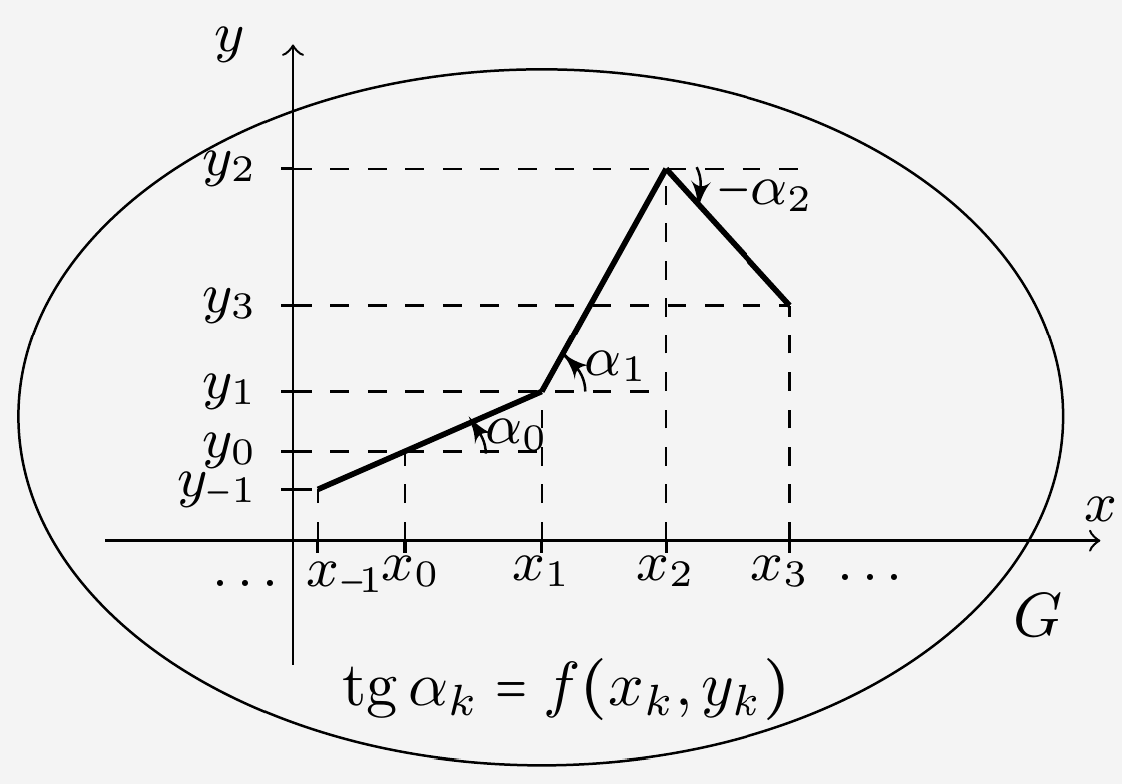
\includegraphics[width=0.445\textwidth]{euler-polylines}
\end{wrapfigure}

Выберем в области $ G $ произвольную точку $ (x_0, y_0) $ и построим в ней отрезок поля направлений столь малой длины, что он целиком лежит в $ G $, начинаясь в какой-то точке $ (x_{-1}, y_{-1}) $ и заканчиваясь в точке $ (x_1, y_1) $ \\
Проведём вправо через точку $ (x_1, y_1) $ и влево через точку $ (x_{-1}, y_{-1}) $ полуотрезки поля, лежащие в $ G $ и заканчивающиеся в точках $ (x_2, y_2) $ и $ (x_{-2}, y_{-2}) $ соответственно, и так далее \\
Этот процесс можно продолжать любое конечное число шагов $ N $, поскольку область $ G $ -- открытое множество \\
График полученной таким образом непрерывной кусоч"-но-линейной функции $ y = \psi(x) $ называется ломаной Эйлера \\
Итак, установлено, что ломаная Эйлера лежит в области $ G $, проходит через точку $ (x_0, y_0) $ и абсциссы её угловых точек равны $ x_j $ ($ j = \ol{-N, N} $)

\begin{definition}
	Рангом дробления ломаной Эйлера назовём число, равное
    $$ \max\limits_{j = \ol{1 - N, N}}\set{x_j - x_{j - 1}} $$
\end{definition}

Формула, реккурентно задающая ломаную Эйлера $ y = \psi(x) $, иммеет вид: $ \psi(x_0) = y_0 $ и далее при $ j = 0, 1, ..., N - 1 $ для любого $ x \in (x_j, x_{j + 1}] $ или при $ j = 0, -1, ..., 1 - N $ для любого $ x \in [x_{j - 1}, x_j) $
\begin{equ}{1.8}
	\psi(x) = \psi(x_j) + f \big( x_j, \psi(x_j) \big)(x - x_j)
\end{equ}
В частности, при $ j = 0 $ отрезок ломаной Эйлера определён для любого $ x \in [x_{-1}, x_1] $ и, делясь на два полуотрезка, проходит через точку $ (x_0, y_0) $ под углом, тангенс которого равен $ f(x_0, y_0) $ \\
Из формулы \eref{1.8} вытекает, что для всякого $ j = \ol{0, N - 1} $ производная $ \psi'(x) = f \big( x_j, \psi(x_j) \big) $ при $ x \in (x_j, x_{j + 1}) $, а в точке $ x_{j + 1} $ она не определна, как и в точках $ x_{j - 1} $ при $ j \le 0 $ \\
Доопределим $ \psi'(x) $ в точках разрыва как левостороннюю производную при $ x > x_0 $ и как правостороннюю производную при $ x < x_0 $, положив
$$ \psi'(x_j) = \psi_{\mp}'(x_j) \liml{x \to x_j^{\mp0}}\frac{\psi(x) - \psi(x_j)}{x - x_j} \qquad (j = \pm 1. ..., \pm N) $$
А при $ j = 0 $ существует полная производная $ \psi'(x_0) = f(x_0, y_0) $ \\
Таким образом, для любого $ x \in (x_j, x_{j + 1}] $ ($ j = 0, 1, ..., N - 1 $) или для любого $ x \in [x_{j - 1}, x_j) $ ($ j = 0, -1, ..., 1 - N $), дифференцируя равенство \eref{1.8} по $ x $, получаем
\begin{equ}{1.9}
    \psi'(x) = f \big( x_j, \psi(x_j) \big), \qquad j \in \set{1 - N, ..., N - 1}
\end{equ}

\subsection{Лемма об \texorpdfstring{$ \veps $}e-решении}

Покажем, что на некотором промежутке всегда можно построить функцию, график которой проходит через заданную точку области $ G $, такую, что при подстановке этой функции в уравнение \eref{1.1} окажется, что разность между левой и правой частями уравнения по модулю не превосходит любого сколь угодно малого наперёд заданного положительного числа

\begin{definition}
    Для всякого $ \veps > 0 $ непрерывная и кусочно-гладкая на отрезке $ [a, b] $ функция $ y = \psi(x) $ называется $ \veps $-решением уравнения \eref{1.1} на $ [a, b] $, если для любого $ x \in [a, b] $ точка $ \big( x, \psi(x) \big) \in G $ и
    \begin{equ}{1.10}
    	\big| \psi'(x) - f \big( x, \psi(x) \big) \big| \le \veps
    \end{equ}
\end{definition}

\begin{lemma}[о ломаных Эйлера в роли $ \veps $-решения]
    Для любой точки $ (x_0, y_0) \in G $ и для любого отрезка Пеано $ \ol{P_h}(x_0, y_0) $ имеем:
    \begin{enumerate}
        \item Для любого $ \delta > 0 $ на $ \ol{P_h} $ можно построить ломаную Эйлера $ y = \psi(x) $ с рангом дробления, не превосходящим $ \delta $, график которой лежит в прямоугольнике $ \ol{R} $ \nimp[из определения отрезка Пеано]
        \item Для любого $ \veps > 0 $ найдётся такое $ \delta > 0 $, что всякая ломаная Эйлера $ y = \psi(x) $ с рангом дробления, не превосходящим $ \delta $, является $ \veps $-решением уравнения \eref{1.1} на $ \ol{P_h}(x_0, y_0) $
    \end{enumerate}
\end{lemma}

\begin{proof}
	\hfill
    \begin{enumerate}
        \item Для произвольной точки $ (x_0, y_0) $ из $ G $ построим прямоугольник $ \ol{R} \sub G $ с центром в $ (x_0, y_0) $ и два лежащих в нём равнобедренных треугольника $ \ol{T^-}, \ol{T^+} $ с общей вершиной в точке $ (y_0, x_0) $ и основаниями, параллельными оси ординат, как это было сделано при построении отрезка Пеано \\
        При этом зафиксируются константы $ a, b, M, h $ \\
        Выберем $ \delta_* < \delta $ так, чтобы число $ \frac{h}{\delta_*} \fed N \in \N $ \\
        Положим $ x_{j + 1} \define x_j + \delta_* $ ($ j = \ol{0, N - 1}) $, тогда $ x_N = x_0 + h $ \\
        Для всякого $ x > x_0 $ будем последовательно строить отрезки ломаной Эйлера $ y = \psi(x) $ с узлами в точках $ x_j $ \\
        Для любого $ j = 0, ..., N $ это сделать возможно, так как модуль тангенса укла наклона каждого отрезка равен $ \big| f \big(x_j, \psi(x_j) \big) \big| $, а тангенсы углов наклона боковых сторон треугольника $ \ol{T^+} $ по построению равны $ \pm M $, где $ M = \max|f(x, y)| $ на компакте $ \ol{R} $ \\
        Поэтому любой отрезок ломаной Эйлера, начиная с первого, не может пересечь боковую стенку $ \ol{T^+} $, а значит, содержится в нём \\
        В результате для всех $ x \in [x_0, x_0 + h] $ точка $ \big( x, \psi(x) \big) \in \ol{T^+} $ и требуемая ломаная Эйлера построена на $ [x_0, x_0 + h] $ \\
        Для левого полуотрезка Пеано всё аналогично
        \item Зафиксируем теперь произвольное положительное число $ \veps $ \\
        Функция $ f(x, y) $ непрерывна на компакте $ \ol{R} $, следовательно, по теореме Кантора $ f $ равномерно непрерывна на нём. По определнию это занчит, что существует такое $ \delta_1 > 0 $, что для любых двух точек $ (x' y') $ и $ (x'', y'') $ из прямоугольника $ \ol{R} $ таких, что $ |x' - x''| \le \delta_1 $ и $ |y' - y''| < \delta_1 $, выполняется неравенство $ |f(x', y') - f(x'', y'')| \le \veps $ \\
        Положим $ \delta \define \min\set{\delta_1, \frac{\delta_1}M} $ и покажем, что для любой ломаной Эйлера $ y = \psi(x) $ с рангом дробления меньшим, чем $ \delta $ на отрезке Пеано $ \ol{P_h}(x_0, y_0) = [x_0 - h, x_0 + h] $, справедливо неравенство \eref{1.10}: \\
        Возьмём любую точку $ x $ из отрезка Пеано, например справа от $ x_0 $ \\
        Найдётся индекс $ j \in \set{0, ..., N - 1} $ такой, что $ x \in (x_j, x_{j + 1}] $, т. е. $ x_j $ -- ближайшая к $ x $ левая угловая точка ломаной Эйлера \\
        Согласно \eref{1.9}
        $$ \psi'(x) - f \big(x, \psi(x) \big) = f \big( x_j, \psi(x_j) \big) - f \big( x, \psi(x) \big) $$
        Оценим близость аргументов функции $ f $: \\
        По выбору $ \delta $ и $ j $ имеем
        $$ |x - x_j| \le \delta \le \delta_1, \qquad |\psi(x) - \psi(x_j)| \undereq{\eref{1.8}} \big| f \big( x_j, \psi(x_j) \big) \big| \cdot |x - x_j| \le M\delta \bdef[\le]\delta \delta_1 $$
        Поэтому из равномерной непрерывности функции $ f $ вытекает, что
        $$ \big| f(x_j, \psi(x_j) \big) - f \big( x, \psi(x) \big) \big| \le \veps $$
        А значит, неравенство \eref{1.10} из определения $ \veps $-решения выполняется на отрезке Пеано
    \end{enumerate}
\end{proof}

\subsection{Лемма Арцела-Асколи}

Пусть последовательность функций $ \seq{h_n(x)}n $ задана на $ [a, b] $

\begin{definition}
    Каждая из функций последовательности $ \seq{h_n(x)}n $ ограничена на $ [a, b] $, если
    $$ \forall n \ge 1 \quad \exist K_n > 0 : \quad \forall x \in [a, b] \quad |h_n(x)| \le K_n $$
\end{definition}

\begin{definition}\label{def:clamp:eq}
    Последовательность $ \seq{h_n(x)}n $ \bt{равномерно} ограничена на отрезке $ [a, b] $, если
    $$ \bm{\exist K > 0} : \quad \forall n \ge 1 \quad \forall x \in [a, b] \quad |h_n(x)| \le K $$
\end{definition}

\begin{definition}
    Каждая из функций последовательности $ \seq{h_n(x)}n $ непрерывна на отрезке $ [a, b] $, значит, согласно теореме Кантора, равномерно непрерывна на $ [a, b] $, если
    $$ \forall \veps > 0 \quad \forall n \ge 1 \quad \exist \delta_n > 0 : \quad \forall x', x'' \in [a, b] \quad \nimp[\bigg(] |x' - x''| \le \delta_n \implies |h_n(x') - h_n(x'')| \le \veps \nimp[\bigg)] $$
\end{definition}

\begin{definition}\label{def:cont:eq}
    Последовательность $ \seq{h_n(x)}n $ \bt{равностепенно} непрерывна на отрезке $ [a, b] $, если
    $$ \forall \veps > 0 \quad \bm{\exist \delta > 0} : \quad \forall n \ge 1 \quad \forall x', x'' \in [a, b] \quad \nimp[\bigg(] |x' - x''| \le \delta \implies |h_n(x') - h_n(x'')| \le \veps \nimp[\bigg)] $$
\end{definition}

\begin{definition}
    Последовательность функций $ \seq{h_n(x)}n $ поточечно сходится к некоторой функции $ h(x) $ на отрезке $ [a, b] $, если
    $$ \forall \veps > 0 \quad \forall x \in [a, b] \quad \exist N_x > 0 : \quad \forall i, j \ge N_x \quad |h_i(x) - h_j(x)| \le \veps $$
\end{definition}

\begin{definition}\label{def:lim:eq}
    Последовательность $ \seq{h_n(x)}n $ \bt{равномерно} сходится к некоторой функции $ h(x) $ на отрезке $ [a, b] $, если
    $$ \forall \veps > 0 \quad \bm{\exist N > 0} : \quad \forall i, j \ge N \quad \forall x \in [a, b] \quad |h_i(x) - h_j(x)| \le \veps $$
\end{definition}

\begin{notation}
	Для любого $ x \in [a, b] $ поточечная сходимость обозначается $ h_n(x) \to h(x) $
\end{notation}

\begin{notation}
    Равномерная относительно $ [a, b] $ сходимость обозначается $ h_n(x) \xrightrightarrows[x \to \infty]{[a, b]} h(x) $
\end{notation}

\begin{remark}
    В определениях \ref{def:clamp:eq} и \ref{def:cont:eq} слова ``равномерно'' и ``равностепенно'' означают, что константы $ K, \delta $ не зависят от выбора $ n $, а в \ref{def:lim:eq} -- что номер $ N $ не зависит от выбора $ x $
\end{remark}

\begin{lemma}[Арцела-Асколи; о существовании равномерно сходящейся подпоследовательности]
    Из любой ограниченной и равностепенно непрерывной на $ [a, b] $ последовательности функций $ \seq{h_n}n $ можно выделить равномерно сходящуюся на $ [a, b] $ подпоследовательность
\end{lemma}

\begin{proof}
	Рациональные числа образуют счётное всюду плотное множество на любом промежутке вещественной прямой \\
    Счётность множества рациональных чисел, расположенных на отрезке $ [a, b] $ означает, что их можно перенумеровать: $ r_1, r_2, ... $ \\
    В точке $ r_1 $ числовая последовательность $ \seq{h_n}n $ по предположению сходится, поэтому из неё можно выбрать сходящуюся подпоследовательность, т. е. существует такая последовательность натуральных чисел
    $$ n^{(1)} = \seq{n_i^{(1)}}i, \qquad n_i^{(1)} < n_{i + 1}^{(1)} $$
    что последовательность значений $ \seq{h_{n_i^{(1)}}(r_1)}i $ сходится \\
    В точке $ r_2 $ последовательность $ \seq{h_{n_i}^{(1)}(r_2)}i $ также ограничена, и из ней можно извлечь сходящуюся подпоследовательность, т. е. у последовательности индексов $ n^{(1)} $ имеется такая подпоследовательность индексов $ n^{(2)} = \seq{n_i^{(2)}}i $, что последовательность значений $ \seq{h_{n_i^{(2)}}(r_2)}i $ тоже сходится. При этом она сходится и в точке $ r_1 $ как подпоследовательность сходящейся последовательности \\
    Продолжаем этот процесс \\
    Введём последовательность индексов $ \seq{n_i^{(i)}}i \quad (n_i^{(i)} < n_{i + 1}^{(i)}) $, где $ n_i^{(i)} $ -- $ i $-й член подпоследовательности $ n^{(i)} $ \\
    Функциональная подпоследовательность $ \seq{h_{n_i}^{(i)}(x)}i $ сходится во всех рациональных точках $ [a, b] $, поскольку в любой рациональной точке $ r_k $ последовательность $ \seq{h_{n_i^{(k)}}(x)}i $ сходится по построению, а любая другая с меньшим верхним индексом является её подпоследовательностью \\
    Покажем, что $ \seq{h_{i_*}(x)}i $, где $ i_* = n_i^{(i)} $ является искомой подпоследовательностью: \\
    Зафиксируем произвольное $ \veps > 0 $ \\
    По условию леммы последовательность $ \seq{h_{i_*}(x)}i $ равностепенно непрерывна, следовательно, по выбранному $ \veps $ найдётся такое число $ \delta > 0 $, что
    $$ \forall i \in \N \quad \forall x', x'' \in [a, b] : \quad \nimp[\bigg(] |x' - x''| < \delta \implies |h_{i_*}(x') - h_{i_*}(x'')| \le \frac\veps3 \nimp[\bigg)] $$
    По построению последовательность функций $ \seq{h_{i_*}(x)}i $ сходится поточечно во всех рациональных точках $ r_k $ из $ [a, b] $ \\
    Поэтому по выбранному $ \veps $ для любого $ k \in \N $ найдётся такой номер $ N_{r_k} > 0 $, что $ |h_{i_*}(r_k) - h_{j_*}(r_k)| \le \faktor\veps3 $ для любых $ i_*, j_* > N_{r_k} $ \\
    Последовательность индексов $ N_{r_1}, N_{r_2}, ..., $ -- счётная, поэтому она может стремиться к бесконечности. Перейти к конечной подпоследовательности позволяет использование появившейся из определения равностепенной непрерывности универсальной константы $ \delta $ и плотности множества рациональных чисел: \\
    Разобьём отрезок $ [a, b] $ на непересекающиеся промежутки, длина которых не превосходит $ \delta $. Пусть их окажется $ l $ штук \\
    Множество рациональных чисел всюду плотно, поэтому в каждом промежутке можно выбрать по рациональному числу: $ r_1^*, ..., r_l^* $ \\
    Пусть $ N = \max\set{N_{r_1^*}, ..., N_{r_l^*}} $, где константы $ N_r $ взяты из определения поточечной сходимости последовательности $ \seq{h_{i_*}(x)}i $ \\
    Возьмём произвольное число $ x \in [a, b] $. Предположим, что оно попало в промежуток с номером $ p $. Тогда для любых $ i_*, j_* > N $ получаем:
    $$ |h_{i_*}(x) - h_{j_*}(x)| \trile |h_{i_*}(x) - h_{i_*}(r_p^*)| + |h_{i_*}(r_p^*) - h_{j_*}(r_p^*)| + |h_{j_*}(r_p^*) - h_{j_*}(x)| \le \veps $$
    так как $ |x - r_p^*| \le \delta $ и верна оценка из определения равномерной сходимости \\
    Итак, для любого $ \veps > 0 $ нашлось такое $ N $, что для любых $ i_*, j_* \ge N $ и $ x \in [a, b] $ справедливо неравенство $ |h_{i_*}(x) - h_{j_*}(x)| \le \veps $
\end{proof}

\begin{remark}
	При выполнении условий леммы Арцела-Асколи она позволяет ``объявить о рождении'' функции $ h(x) $, определённой на отрезке $ [a, b] $ и предельной для некоторой подпоследовательности функций $ h_n(x) $ \\
    При этом, по теореме Стокса-Зайделя предельная функция непрерывна на $ [a, b] $
\end{remark}

\begin{note}
	Теорема Стокса-Зайделя -- некоторое обобщение формулы Ньютона-Лейбница
\end{note}

\subsection{Теорема о существовании решения ВЗК}

Докажем теорему \ref{th:Peano}:

\begin{theorem}{Пеано; о существовании внутреннего решения}
    Пусть правая часть уравнения \eref{1.1} непрерывна в области $ G $ \\
    Тогда для любой точки $ (x_0, y_0) \in G $ и для любого отрезка Пеано $ \ol{P_h}(x_0, y_0) $ существует по крайней мере одно решение задачи Коши уравнения \eref{1.1} с начальными данными $ x_0, y_0) $, определённое на $ \ol{P_h}(x_0, y_0) $
\end{theorem}

\begin{proof}
    Возьмём произвольную точку $ (x_0, y_0) $ из области $ G $ и построим какой-либо отрезок Пеано $ \ol{P_h}(x_0, y_0) $ \\
    Выберем произвольную последовательность положительных чисел $ \veps_n $, стремящуюся к нулю при $ n \to \infty $ \\
    Тогда по лемме об $ \veps $-решении для всякого $ n $ можно построить ломаную Эйлера $ \psi_n(x) $, проходящую через точку $ (x_0, y_0) $, определённую на $ \ol{P_h}(x_0, y_0) $ и являющуюся $ \veps_n $-решением уравнения \eref{1.1} на отрезке $ \ol{P_j}(x_0, y_0) $ \\
    Поэтому для любых $ n \in \N $ и $ x \in \ol{P_h}(x_0, y_0) $ точка $ \bigg( x, \psi_n(x) \bigg) \in \ol{R} $ и выполняется неравенство \eref{1.10} $ |\psi_n'(x) - f \big( x, \psi_n(x) \big) | < \veps_n $ \\
    Покажем, что последовательность ломаных Эйлера $ \seq{\psi_n(x)}n $ на отрезке Пеано удовлетворяет лемме Арцела-Асколи \\
    Последовательность $ \seq{\psi_n(x)}n $ равномерно ограничена, так как график любой функции $ y = \psi_n(x) $ лежит в прямоугольнике $ \ol{R} $, а значит, $ |\psi_n(x)| \le |y_0| + b $ для любого $ x \in [x_0 - h, x_0 + h] $ \\
    Для доказательства равностепенной непрерывности зафиксируем произвольное $ \veps > 0 $ \\
    Положим $ \delta = \faktor\veps{M} $, где $ M = \max\limits_{(x, y) \in \ol{R}}|f(x, y)| $ \\
    Тогда для любых $ n \in \N $ и $ x', x'' \in \ol{P_h}(x_0, y_0) $ таких, что $ |x'' - x'| \le \delta $, получаем:
    \begin{multline*}
        |\psi_n(x'') - \psi_n(x')| = \bigg| \dint[s]{x_0}{x''}{\psi_n'(s)} - \dint[s]{x_0}{x'}{\psi_n'(s)} \bigg| = \bigg| \dint[s]{x'}{x''}{\psi_n'(s)} \underset{\eref{1.9}}\le \\
        \le \bigg| \dint[s]{x'}{x''}{\max\limits_{j = 1 - N, ..., N - 1} \big| f \big( x, \psi_n(x_j) \big) \big|} \bigg| \le M|x'' - x'| \le M\delta = \veps
    \end{multline*}
    Действительно, интегрируя кусочно-постоянную функцию $ \psi'(x) $ по $ s $ от $ x_0 $ до $ x $, для любого $ x \in [x_{-N}, x_N] $ имеем: $ \psi(x) = \psi(x_0) + \dint[s]{x_0}x{\psi'(s)} $, где
    $$ \dint[s]{x_0}x{\psi(s)} = \sum_{k = 0}^{j - 1} \dint[s]{x_k}{x_{k + 1}}{\psi'(s)} + \dint[s]{x_j}x{\psi'(s)}, \qquad x \in (x_j, x_{j + 1}], \quad j \in \set{0, ..., N - 1} $$
    $$ \dint[s]{x_0}x{\psi'(s)} = \sum_{k = j + 1}^{-1} \dint[s]{x_{k + 1}}{x_k}{\psi'(s)} + \dint[s]{x_{j + 1}}x{\psi'(s)}, \qquad x \in [x_j, x_{j + 1}), \quad j \in \set{-N, ..., -1} $$
    В результате последовательность ломаных Эйлера $ \psi_n(x) $ удовлетворяет условиям леммы Арцела-Асколи, и из неё можно выделить равномерно сходящуюся подпоследовательность $ \seq{\psi_{i_*}(x)}{i_*} $ \\
    Пусть $ \psi_{i_*} \xrightrightarrows[i_* \to \infty]{x \in \ol{P_h}} \vphi(x) $ \\
    Тогда, согласно замечанию \nimp[после леммы Арцела-Асколи] функция $ y = \vphi(x) $ непрерывна на отрезке Пеано \\
    Поскольку $ \psi_{i_*}(x) $ по построению является $ \veps_{i_*} $-решением, из неравенства \eref{1.10} вытекает, что
    $$ \foral x \in \ol{P_h}(x_0, y_0) \quad \foral i_* \in \N : \quad \psi_{i_*}'(x) = f \big( x, \psi_{i_*}(x) \big) + \Delta_{i_*}(x), \qquad |\Delta_{i_*}(x)| \le \veps_{i_*} $$
    Интегрируя это равенство по $ s $ от $ x_0 $ до $ x $ получаем:
    \begin{equ}{1.11}
        \psi_{i_*}(x) - \psi_{i_*}(x_0) = \dint[s]{x_0}x{f \big( s, \psi_{i_*}(s) \big)} + \dint[s]{x_0}x{\Delta_{i_*}(s)}
    \end{equ}
    причём $ \psi_{i_*}(x_0) = y_0 $ и $ \bigg| \dint[s]{x_0}x{\Delta_{i_*}(s)} \bigg| \le \veps_{i_*}|x - x_0| \underarr{i_* \to \infty} 0 $, так как $ |x - x_0| \le h $ \\
    Кроме того, $ f \big( s, \psi_{i_*}(s) \big) \xrightrightarrows[i_* \to \infty]{s \in \ol{P_h}} f \big( s, \vphi(s) \big) $, поскольку любая точка $ \big( s, \psi_{i_*}(s) \big) \in \ol{R} $ и $ f(x, y) $ по теореме Кантора равномерно непрерывна на $ \ol{R} $
    \begin{statement}
        Поэтому можно осуществить предельный переход под знаком интеграла:
        $$ \dint[s]{x_0}x{f \big( s, \psi_{i_*}(s) \big)} \underarr{i_* \to \infty} \dint[s]{x_0}x{f \big( s, \vphi(s) \big)} $$
    \end{statement}
    \begin{proof}
        Действительно, зафиксируем произвольное число $ \veps > 0 $ \\
        Из равномерной непрерывности функции $ f(x, y) $ на компакте $ \ol{R} $ вытекает, что по выбранному $ \veps $ найдётся такое $ \delta $, что для любых $ (x, \vawe{y}), (x, \hat{y}) \in \ol{R} $ выполнено $ |\hat{y} - \vawe{y}| < \delta \implies |f(x, \hat{y}) - f(x, \vawe{y})| < \faktor\veps{h} $ \\
        Теперь из равномерной относительно $ x \in [x_0 - h, x_0 + h] $ сходимости последовательности функций $ \psi_{i_*}(x) $ к функции $ \vphi(x) $ вытекает, что для найденного $ \delta $ существует такой номер $ N $, что $ |\psi_{i_*}(x) - \vphi(x)| < \delta $ для любых $ i_* \ge N $ и $ x \in \ol{P_h}(x_0, y_0) $, причём графики $ y = \psi_{i_*}(x) $ и $ y = \vphi(x) $ по доказанному лежат в $ \ol{R} $ \\
        Следовательно, $ \bigg| f \big(x, \psi_{i_*}(x) \big) - f \big( x, \vphi(x) \big) \bigg| < \faktor\veps{h} $, и при $ i_* \ge N $ имеем:
        $$ \bigg| \dint[s]{x_0}x{f \big( s, \psi_{i_*}(s) \big)} - \dint[s]{x_0}x{f \big( s, \vphi(s) \big)} \bigg| \le \bigg| \dint[s]{x_0}x{\big| f \big(s, \psi_{i_*}(s) \big) - f \big( s, \vphi(s) \big) \big|} \bigg| < \frac{\veps|x - x_0|}h \le \veps $$
    \end{proof}
    Перезодя в обеих частях равенств \eref{1.11} к пределу при $ i_* \to \infty $, получаем тождество \eref{1.2}:
    $$ \vphi(x) \overset{[x_0 - h, x_0 + h]}\equiv \vphi(x_0) + \dint[s]{x_0}x{f \big(s, \vphi(s) \big)} $$
    Поэтому, согласно лемме о записи решения в интегральном виде, предельная функция $ y = \vphi(x) $ является решением ВЗК$ (x_0, y_0) $ уравнения \eref{1.1} на отрезке Пеано $ [x_0 - h, x_0 + h] $
\end{proof}

\begin{remark}
	Теорема Пеано не даёт информации о количестве решений, проходящих через заданную точку области $ G $
\end{remark}

\begin{remark}
	Для точек неединственности существуют решения, которые нельзя приблизить ломанными Эйлера
\end{remark}

\section{Существование решения граничной задачи Коши}

В этом параграфе будут указаны условия, при которых существует решение ГЗК уравнения \eref{1.1}, поставленной в произвольной точке $ (x_0, y_0) \in \hat{G} \sub \partial G $, и условия, при которых такое решение отсутсвует. Поставленная задача решается путём выделения тех случаев, в которых возможно построение аналогов труегольника и отрезка Пеано, с последующим применением метода ломаных Эйлера. \\
Для упрощения обозначений и формул, используемых в дальнейшем при решении граничной задачи Коши, НУО будем считать, что задача всегда ставится в начале координат и функция $ f $ там равна нулю, т. е. уравнение \eref{1.1} имеет вид
\begin{equ}{1.12}
	y' = f_0(x, y)
\end{equ}
где функция $ f_0 $ определена и непрерывна на множестве $ \vawe{G} = G \cup \hat{G} $, точка $ O = (0, 0) \in \vawe{G} $, $ f_0(0, 0) = 0 $ и поставлена граничная задача Коши с начальными данными $ 0, 0 $
\begin{proof}[НУО]
    В самом деле, пусть для уравнения \eref{1.1} $ y' = f(x, y) $ задача Коши поставлена в точке $ (x_0, y_0) \in \hat{G} $. Тогда замена
    $$ x = u + x_0, \qquad y = v + y_0 + f(x_0, y_0)(x - x_0) $$
    сводит уравнение \eref{1.1} к уравнению $ v' = f_0(u, v) $, в котором
    $$ f_0(u, v) = f \bigg( u + x_0, v + f(x_0, y_0)u + y_0 \bigg) $$
    При этом для $ x = x_0 $, $ y = y_0 $ получаем:
    $$ u = u_0 = 0, \qquad v = v_0 = 0, \qquad f_0(0, 0) = 0 $$
\end{proof}

\subsection{Граничные кривые и порождаемые ими множества}

Ключевую роль для существования или отсутсвия решения ГЗК уравнения \eref{1.12} будет играть структура граничного множества в $ \hat{G} $ в малой окрестности точки $ O $ и значения функции $ f_0 $ на нём, а также расположение всего множества $ \vawe{G} $ по отношению к оси абсцисс

\begin{definition}
    Функцию $ y = b_{a, u}^+(x) $ заданную на отрезке $ [0, a] $ будем называть верхнеграничной, если для неё выполняются следующие пять условий:
    \begin{enumerate}
        \item $ b_{a, u}^+(x) \in \Cont[1]{[0, a]} $
        \item $ b_{a, u}^+(0) = 0 $
        \item\label{def:ruf:en:3} $ b_{a, u}^+{}'(0) \ge 0 $
        \item\label{def:ruf:en:4} $ b_{a, u}^+ $ вогнута на $ [0, a] $, если $ b_{a, u}^+{}'(0) = 0 $
        \item Правая верхнеграничная кривая $ \gamma_{a, u}^+ = \set{x \in [0, a], \quad y = b_{a, u}^+(x)} \sub \hat{G} $
    \end{enumerate}
\end{definition}

\begin{note}
    Условие \ref{def:ruf:en:3} допускает случай, когда $ b_{a, u}^+{}'(0) = +\infty $ \\
    В условии \ref{def:ruf:en:4} вогнутость понимается в нестрогом смысле, т. е. допускается тождество $ b_{a, u}^+(x) \equiv 0 $
\end{note}

Аналогично вводится правая нижнеграничная функция $ y = b_{a, l}^+(x) $, и правая нижнеграничная кривая $ \gamma_{a, l}^+ $ -- график $ b_{a, l}^+(x) $. Только в условии \ref{def:ruf:en:3} предполагаем, что $ b_{a, l}^+{}'(0) \le 0 $, и допускаем случай, когда $ b_{a, l}^+{}'(0) = -\infty $, а в условии \ref{def:ruf:en:4} предполагаем, что $ b_{a, l}^+(x) $ выпукла \\
Введём две ключевые константы:
$$ \tau_u = \half[b_{a, u}^+{}'(0)], \qquad \tau_u = 1 \text{, если } b_{a, u}^+{}'() = +\infty $$
$$ \tau_l = -\half[b_{a, l}^+{}'(0)], \qquad \tau_l = -1 \text{, если } b_{a, l}^+{}'(0) = -\infty $$
НУО будем считать, что выполняются условия:
\begin{equ}{1.13+}
    \begin{cases}
        b_{a, u}^+(a) \le a \quad \text{при } \tau_u = 0 \\
        \foral x \in [0, a] \quad b_{a, u}^+{}'(x) \ge \tau_u \quad \text{при } \tau_u > 0 \\
        -b_{a, l}^+(a) \le a \quad \text{при } \tau_l = 0 \\
        \foral x \in [0, a] \quad -b_{a, l}^+{}'(x) \ge \tau_l \quad \text{при } \tau_l > 0
    \end{cases}
\end{equ}
поскольку непостредственно из определения вытекает, что для любой правой граничной функции $ b_a^+(x) $ функция $ b_{\breve{a}}^+(x) $, являющаяся её сужением на произвольный отрезок $ [a, \breve{a}] $ с $ \breve{a} < a $, остаётся правой граничной. \\
В результате $ \gamma_{a, u}^+ $ -- гладкая кривая из $ \hat{G} $, параметризованная неубывающей с учётом \eref{1.13+} функцией $ b_{a, u}^+(x) $. Она расположена в первой четверти и содержит точку $ O $. $ \gamma_{a, l}^+ $ -- гладкая кривая из $ \hat{G} $, параметризованная невозрастающей функцией $ b_{a, l}^+(x) $. Она расположена в четвёртой четверти и содержит точку $ O $ \\
Для всякого $ c > 0 $ рассмотрим правую $ c $-\textit{окрестность} \nimp[(это не окрестность -- она не открыта)] точки $ O $:
$$ N_c^+ \define \set{(x, y) | x \in (0, c], \quad |y| \le c} $$
В прямоугольнике $ N_c^+ $ длина верхней стороны выбирается так, чтобы каждая ``выходящая'' из точки $ O $ правая граничная кривая, при наличии хотя бы одной, имела пересечение с одной из его сторон. При этом ``поведение'' гранчных кривых после первого попадания на границу $ N_c^+ $ интереса не представляет. \\
Любое последующее уменьшение $ c $ ситуацию не меняет, разве что отсекаются части граничных кривых, попавших в прямоугольник снаружи. \\
В частности, неравенства $ b_{a, u}^+(a) \le a $ или $ -b_{a, l}^+(a) \le a $ из \eref{1.13+} при всех $ c \le a $ гарантируют пересечение правых граничных кривых $ \gamma_a^+ $ именно с боковой стороной прямоугольника $ N_c^+ $. \\
Всегда в дальнейшем, ``обрезая'' при необходимости кривые $ \gamma_a^+ $, будем считать, что правый конец $ \big( a, b_a^+(a) \big) $ любой из них -- это первая точка выхода граничной кривой на границу прямоугольника $ N_c^+ $ \\
Выделим для уравнения \eref{1.12} четыре варианта расположения граничных кривых в малой окрестности точки $ O $ при $ x > 0 $:
\begin{definition}
	Будем говорить, что
    \begin{enumerate}
        \item реализуется случай $ (W^+) $, если
        $$ \exist c_W > 0 : \quad W_{c_W}^+ \cap \hat{G} = \O, \qquad W_{c_W}^+ = N_{c_W}^+ $$
        \item реализуется случай $ (U^+) $, если
        $$ \exist c_U > 0 : \quad U_{c_U}^+ \cap \hat{G} = \gamma_{a, u}^+ \setminus \set{O} $$
        $$ U_{c_U}^+ \define \set{(x, y) | \bigg( x \in (0, a], \quad -c_u \le y \le b_{a, u}^+(x) \bigg) \cup \bigg( x \in (a, c_U], \quad y \le c_U \bigg)} $$
        \item реализуется случай $ (O^+) $, если
        $$ \exist c_O > 0 : \quad O_{c_O}^+ \cap \hat{G} = \gamma_{a, l}^+ \setminus \set{O} $$
        $$ O_{c_O}^+ \define \set{(x, y) | \bigg( x \in (0, a], \quad b_{a, l}^+(x) \le y \le c_O \bigg) \cup \bigg( x \in (a, c_O], \quad |y| \le c_O \bigg)} $$
        \item реализуется случай $ (B^+) $, если
        $$ \exist c_B > 0 : B_{c_B}^+ \cap \hat{G} = \big( \gamma_{a, u}^+ \cup \gamma_{a, l}^+ \big) \setminus \set{O}, \qquad B_{c_B}^+ \define U_{c_B}^+ \cap O_{c_B}^+ $$
    \end{enumerate}
\end{definition}

\begin{notation}
    $ (X^+) $ и $ (X_{c*}^+) $ будут обозначать далее, что реализуется любой из четырёх описанных выше случаев на соответствующем множестве
\end{notation}

В случае $ (X^+) $ или $ (X_{c*}^+) $ имеет место одна из двух возможностей:
\begin{enumerate}
    \item $ X_{c*}^+ \cap G \ne \O $, что равносильно тому, что $ X_{c*}^+ $ без входящих в него граничных кривых лежит в $ G $
    \item $ X_{c*}^+ \cap G = \O $
\end{enumerate}

В результате случай $ (X^+) $ в зависимости от расположения множества $ X_{c*} $ распадается на два подслучая, которые будем обозначать $ (X_1^+) $ и $ (X_2^+) $ \\
А дополнительный индекс $ >, =, < $, при его наличии в обозначении любого из шести возникших случаев (кроме $ (W_1^+) $ и $ (W_2^+) $), будет уточнять знак производной соответсвующих правых граничных функций в нуле \\
В итоге, получаются случаи:
\begin{enumerate}
    \item[$ \bm{U_1^+} $:] $ (U_{c_U}^+ \setminus \gamma_{a, u}^+) \sub G $, два подслучая:
    \begin{enumerate}
        \item[$ \bm{U_1^{+, >}} $:] $ b_{a, u}^+{}'(0) > 0 $
        \item[$ \bm{U_1^{+, =}} $:] $ b_{a, u}^+{}'(0) = 0 $
    \end{enumerate}
    \item[$ \bm{U_2^+} $:] $ U_{c_U}^+ \cap G = \O $, подслучаи те же
    \item[$ \bm{O_1^+} $:] $ (O_{c_O}^+ \setminus \gamma_{a, l}^+) \sub G $, два подслучая:
    \begin{enumerate}
        \item[$ \bm{O_{1, <}^+} $:] $ b_{a, l}^+{}'(0) < 0 $
        \item[$ \bm{O_{1, =}^+} $:] $ b_{a, l}^+{}'(0) = 0 $
    \end{enumerate}
    \item[$ \bm{O_2^+} $:] $ O_{c_O}^+ \cap G = \O $, подслучаи те же
    \item[$ \bm{B_1^+} $:] $ \bigg(B_{c_B}^+ \setminus (\gamma_{a, u}^+ \cup \gamma_{a, l}^+) \bigg) \sub G $, четыре подслучая:
    \begin{enumerate}
        \item[$ B_{1, <}^{+, >} $:] $ b_{a, u}^+{}'(0) > 0, \quad b_{a, l}^+{}'(0) < 0 $
        \item[$ B_{1, =}^{+, =} $:] $ b_{a, u}^+{}'(0) = 0, \quad b_{a, l}^+{}'(0) = 0 $
        \item[$ B_{1, =}^{+, >} $:] $ b_{a, u}^+{}'(0) > 0, \quad b_{a, l}^+{}'(0) = 0 $
        \item[$ B_{1, <}^{+, =} $:] $ b_{a, u}^+{}'(0) = 0, \quad b_{a, l}^+{}'(0) < 0 $
    \end{enumerate}
    \item[$ \bm{B_2^+} $:] $ B_{c_B}^+ \cap G = \O $, подслучаи те же
\end{enumerate}

\begin{figure}[!h]
    \begin{subcaptionblock}{\textwidth}
        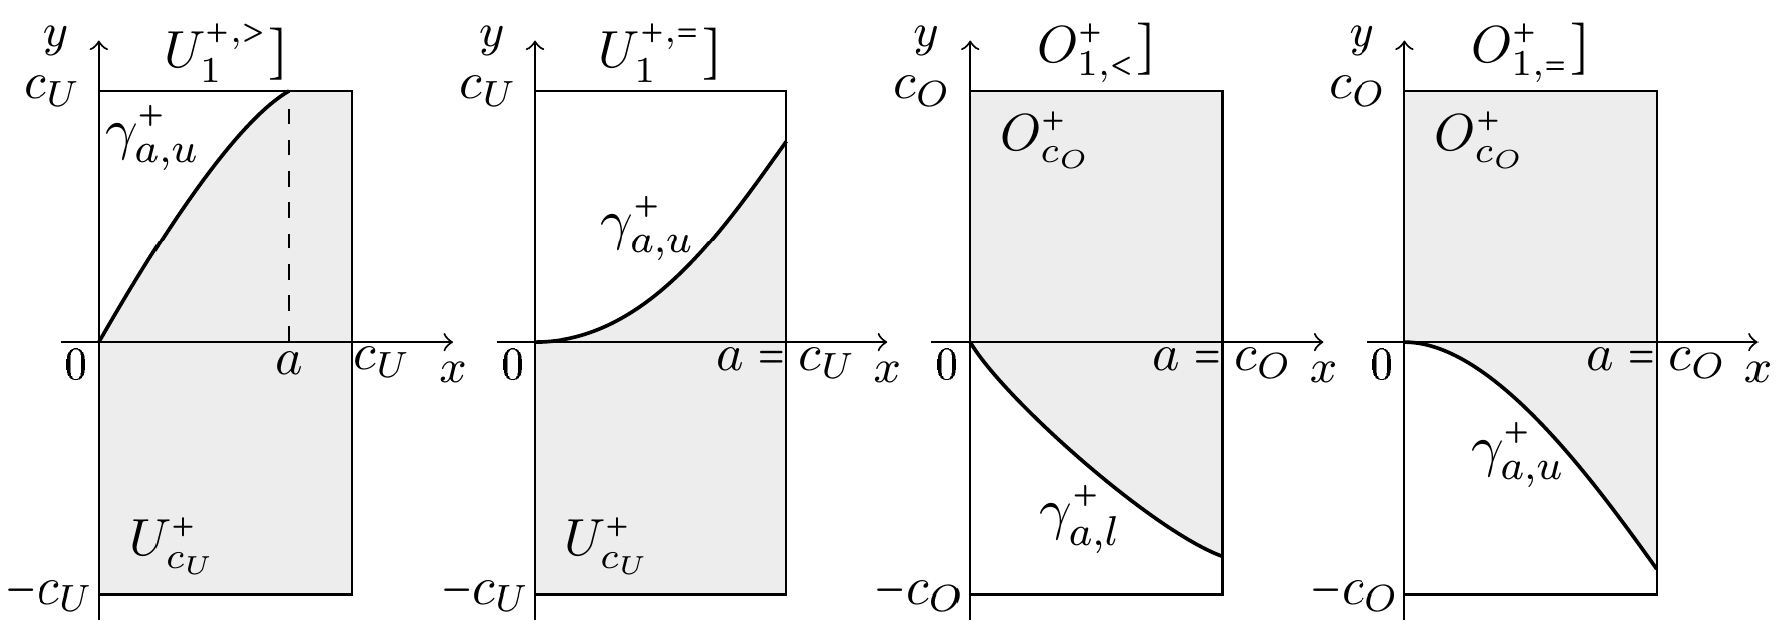
\includegraphics[width=0.99\textwidth]{boundary_curves_1}
    \end{subcaptionblock}
    \begin{subcaptionblock}{\textwidth}
    	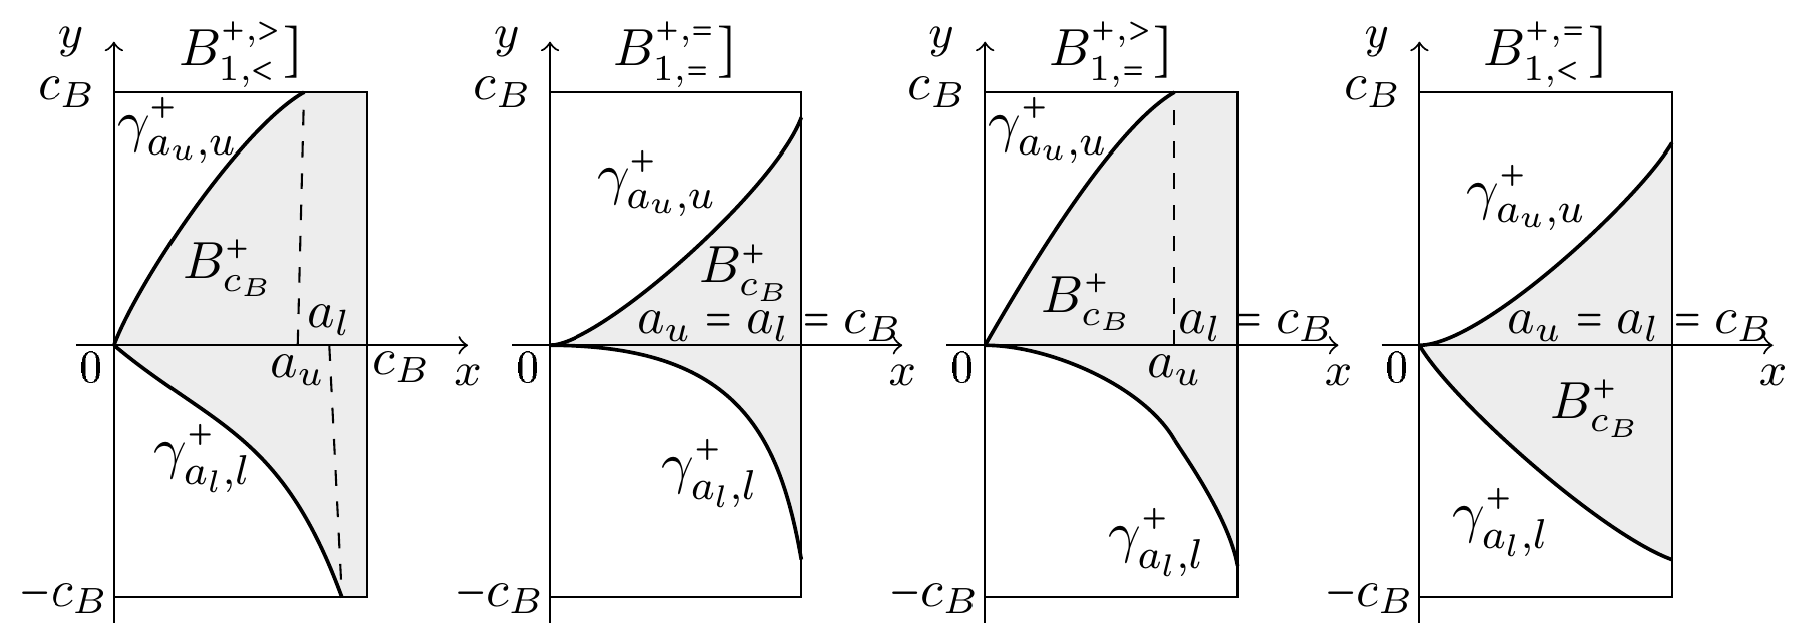
\includegraphics[width=0.99\textwidth]{boundary_curves_2}
    \end{subcaptionblock}
\end{figure}

\begin{remark}
	Прямоугольник $ N_c^+ $ может содержать более одной нижнеграничной и более одной нижнеграничной кривой. Но наличие или отсутсвие граничных кривых в $ N_c^+ $ вне множества $ X_c^+ $ не влияет на существование решения ГЗК($ x_0, y_0 $)
\end{remark}

\begin{remark}
    При наличии в $ N_c^+ $ единственной граничной кривой, дежащей на оси абсцисс, будем считать, что имеет место случай $ (U_1^{+, =} $) с $ b_{a, u}^+ \equiv 0 $, \nimp[а не $ (O_{2, =}^+) $ с $ b_{a, l}^+ \equiv 0 $]. То же касается случаев $ (O_{1, =}^+) $ и $ (U_2^{+, =}) $
\end{remark}

\subsection{Граничный треугольник и граничный отрезок Пеано}

Для доказательства существования решения ГЗК($ O = (0, 0) \in \hat{G} $), график которого расположен, скажем, в правой полуплоскости, в первую очередь следует выделить так называемый правый граничный отрезк Пеано $ \ol{P_h+}^+(O) = [0, h^+] $ ($ h^+ > 0 $). А для этого необходимо построить правый граничный треугольник $ \ol{T_b^+} $, во многом аналогичный треугольнику $ \ol{T^+} $ из определения отрезка Пеано для внутренней задачи Коши, высота которого как раз и здадаёт константу $ h^+ $. Осуществить это удаётся в случаях $ (N_1^+), (U_1^+), (O_1^+), (B_1^+) $ при дополнительных предположениях о поведении функции $ f_0 $ на тех граничных кривых, которые в нуле имеют нулевую производную \\
При построении будет использоваться непрерывность функции $ f_0(x y) $ в граничной точке $ O $, где по условию $ f_0 $ равна нулю, означающая, что
\begin{equ}{1.14}
    \forall \tau > 0 \quad \exist \delta_\tau > 0 : \quad \forall (x, y) \in \ol{V}_{\delta_\tau} \cap \vawe{G} \quad |f_0(x, y)| \le \tau, \qquad \ol{V}_{\delta_\tau} \define \set{(x, y) | {} |x| \le \delta_\tau, \quad |y \le \delta_\tau}
\end{equ}
В простейшем случае $ (W_1^+) $, когда весь прямоугольник $ N_{c_W}^+ $ лежит в $ G $ (граничные кривые в $ c_W $-о\-крест\-нос\-ти точки $ O $ могут быть расположены только на оси ординат или в левой полуплоскости), правый треугольник $ \ol{T_b^+} $ и правый отрезок Пеано $ [0, h^+] $ строятся стандартно: \\
Выберем, например, $ \tau = 1 $. Тогда, согласно \eref{1.14} найдётся $ \delta_1 > 0 $ такое, что $ |f_0(x, y)| \le 1 $ на множестве $ \ol{V}_{\delta_1} \cap \vawe{G} $ \\
Положим $ \vawe{c} \define \min\set{c_W, \delta_1} $ \\
Построим в прямоугольнике $ N_{\vawe{c}}^+ $, не содержащем граничных кривых, с добавленной к нему точкой $ O $, прямоугольный равнобедренный треугольник $ \ol{T_b}^+ $ с вершинами в точках $ (0, 0), (\vawe{c}, \vawe{c}), (\vawe{c}, -\vawe{c}) $. Тогда длина его высоты $ h^+ $ равна $ \vawe{c} $, а его боковые стороны имеют углы наклона, равные $ \pm \frac\pi4 $, поэтому любая ломаная Эйлера, ``выпущенная'' из начала координат, в силу выбора $ \tau = 1 $ в \eref{1.14} будет продолжима до точки $ (h^+, y_*) $, лежащей на основании $ \ol{T_b^+} $, совпадающем в данном случае с правой стороной $ N_{\vawe{c}}^+ $ \\
Похожие построения будут проведены для случаев $ (U_1^{+, >}) $, $ (O_{1, <}^+) $, $ (B_{1, <}^{+, >}) $ \\
В остальных пяти случаях из-за того, что в каждом производная хотя бы одной из граничных функций в нуле равна нулю, может оказаться, что не все ломанные Эйлера могут быть продолжены до основания любого ``классического'' правого треугольника Пеано. Дело в том, что часть граничной кривой вблизи точки $ O $ такой граничной функции будет обязательно лежать внутри треугольника со сколь угодно малым углом при вершине $ O $. Поэтому может найтись точка на этой части границы, в которой модуль угла наклона касательной будет меньше значения функции $ f_0 $ в этой точке, а значит, при попадании ломаной в эту точку её продолжение вправо должно будет покинуть множество $ \vawe{G} $, что невозможно

\begin{figure}[!h]
    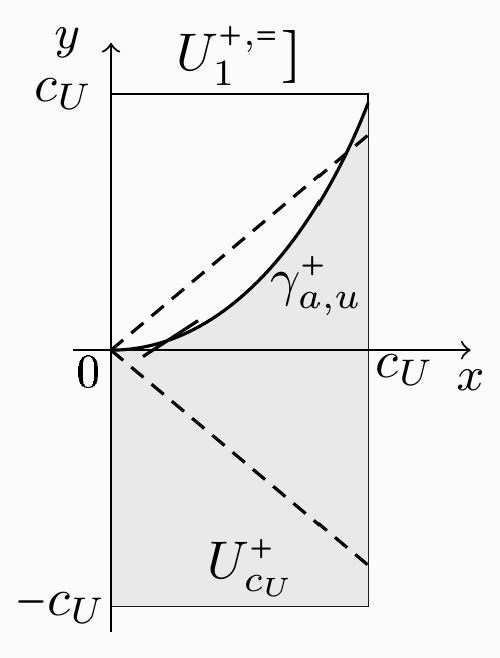
\includegraphics[scale=0.3]{boundary_curves_3}
\end{figure}

\begin{note}
    На рисунке описанная ситуация возникает в случае $ (U_1^{+, =}) $ \\
    Действительно, каким бы малым ни выбрать $ \tau $ в формуле \eref{1.14}, вссегда найдётся константа $ c \le \min\set{c_I, \delta_\tau} $ такая, что в прямоугольнике $ N_{\vawe{c}^+} $ с $ \vawe{c} = \min\set{c_U, \delta_\tau} $ часть правой верхнеграничной кривой $ \gamma_{\vawe{c}, u}^+ $, примыкающая к точке $ O $, будет лежать под верхней боковой стороной прямоугольника $ T_b^+ $, имеющей угол наклона $ \arctg \tau $. Поэтому ломаная Эйлера, которая не может покидать $ \vawe{G} $, попадая в какой-то точке $ \big( x_*, b_{\vawe{c}, u}^+(x_*) \big) $ ($ x_* < \vawe{c} $) на $ \gamma_{\vawe{c}, u}^+ $, не сможет быть продолжена вправо, если вы этой точке отрезок поля направлений будет иметь угол наклона, не превосходищий $ \arctg \tau $, но больший угла наклона касательной к $ \gamma_{\vawe{c}, u}^+ $
\end{note}

Для устранения этой проблемы во всех точках кривых $ \gamma_{a, u}^+ $ и $ \gamma_{a, l}^+ $ введём ограничения на функцию $ f_0 $ в случаях $ (U_1^{+, =}), (O_{1, =}^+), (B_{1, =}^{+, =}), (B_{1, =}^{+, >}) $ и $ (B_{1, <}^{+, =}) $:
\begin{equ}{1.15+}
	\forall x \in (0, a] \quad
    \begin{cases}
        f_0 \big( x, b_{a, u}^+(x) \big) \le b_{a, u}^+{}'(x), \qquad \text{если } b_{a, u}^+{}'(0) = 0 \\
        f_0 \big( x, b_{a, l}^+(x) \big) \ge b_{a, l}^+{}'(x), \qquad \text{если } b_{a, l}^+{}'(0) = 0
    \end{cases}
\end{equ}
означающие, что в любой точке $ \gamma_{a, u}^+ $ и $ \gamma_{a, l}^+ $ правый полуотрезок поля направлений уравнения \eref{1.12} направлен внутрь или по границе области $ G $ \\
Построим отрезок Пеано в восьми случаях $ (X_1^+) $:
\begin{enumerate}
    \item[$ \bm{U_1^{+, >}} $.] Пусть $ \vawe{c} = \min\set{c_U, \delta_{\tau_u}} $, где $ \tau_u $ из \eref{1.13+}, а $ \delta_{\tau_u} $ задана в \eref{1.14}. \\
    Тогда $ U_{\vawe{c}}^+ \setminus \gamma_{\vawe{a}, u}^+ \sub G $, где $ \vawe{a} $ -- точка пересечения $ \gamma_{a, u}^+ $ с верхней или боковой $ (\vawe{a} = \vawe{c} $) границей $ N_{\vawe{c}}^+ $, $ |f_0(x, y)| \le \tau_u $ при $ (x, y) \in U_{\vawe{c}}^+ $ и $ h^+ = \vawe{a} $ \\
    Геометрически надо из точки $ O $ провести лучи с тангенсами углов наклона, равными $ \pm \tau $, до пересечения с вертикальной прямой $ x \equiv \vawe{a} $. В полученном равнобедренном треугольнике $ \ol{T_b^+} $ высота $ h_\Delta^+ = \vawe{a} $. При этом $ \ol{T_b^+} \setminus \set{O} \sub U_{\vawe{c}}^+ $ (и расположен под кривой $ \gamma_{\vawe{a}, u}^+ $) в силу выбора $ \vawe{a} $, так как согласно \eref{1.13+} верно неравенство $ b_{\vawe{a}, u}^+(x) \ge \tau_ux $ при $ x \in [0, \vawe{a}] $
    \item[$ \bm{U_1^{+, =}} $.] Пусть в \eref{1.14} $ \tau = 1 $, $ \vawe{c} = \min\set{c_U, \delta_1} $. Тогда $ U_{\vawe{c}}^+ \setminus \gamma_{\vawe{a}, u}^+ \sub G $, причём $ \vawe{a} = \vawe{c} $, так как правый конец $ \gamma_{\vawe{a}, u}^+ $ с учётом \eref{1.13+} заканчивается на боковой стороне $ N_{\vawe{c}}^+ $, $ |f_0(x, y)| \le 1 $ при $ (x, y) \in U_{\vawe{c}}^+ $ и $ h^+ = \vawe{c} $ \\
    Геометрически надо соединить точки $ O $ и $ (\vawe{c}, -\vawe{c}) $. Тогда полученный отрезок вместе с кривой $ \gamma_{\vawe{a}, u}^+ $ и отрезком боковой стороны $ N_{\vawe{c}}^+ $ образует криволинейный треугольник $ \ol{T_b^+} $ с высотой $ h_\Delta^+ = \vawe{c} $, при этом $ \ol{T_b^+} \setminus O \sub U_{\vawe{c}}^+ $
    \item[$ \bm{O_{1, <}^+}, \bm{O_{1, =}^+} $.] Аналогично, только на рисунке для случая $ (O_{1, <}^+) $ кривая $ \gamma_{\vawe{a}, l}^+ $, над которой расположен треугольник $ \ol{T_b^+} $, пересекается не с нижней, а с боковой стороной прямоугольника $ N_{\vawe{c}^+} $

    \begin{figure}[!h]
        \centering
    	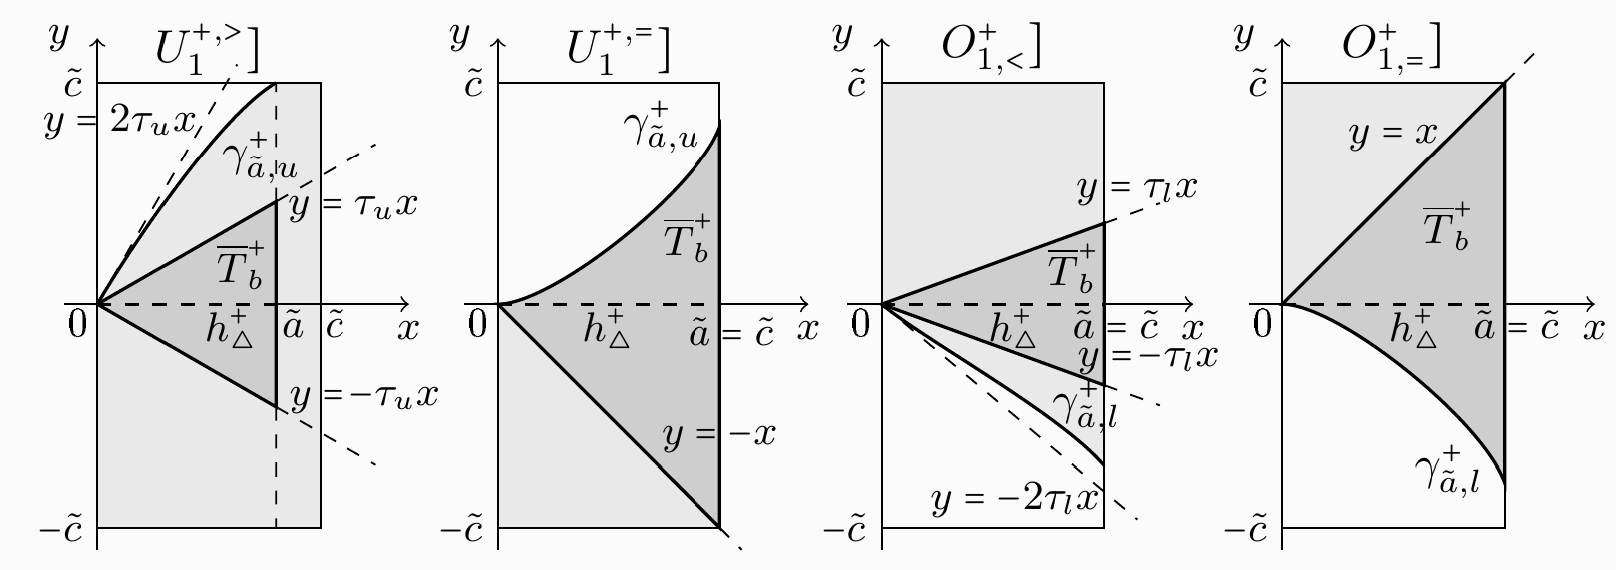
\includegraphics[width=0.9\textwidth]{boundary_curves_4}
    \end{figure}

    \item[$ \bm{B_{1, <}^{+, >}} $.] Пусть $ \vawe{c} = \min\set{c_B, \delta_{\vawe{\tau}}} $, где $ \vawe\tau = \min\set{\tau_u, \tau_l} $ (см. \eref{1.13+}). Тогда $ B_{\vawe{c}^+} \setminus \big( \gamma_{a_u, u}^+ \cup \gamma_{a_l, l}^+ \big) \sub \gamma $, $ |f_0(x, y)| \le \vawe\tau $ при $ (x, y) \in B_{\vawe{c}}^+ $ и $ h^+ = \vawe{a} = \min\set{a_u, a_l} $ \\
    Геометрически надо из точки $ O $ провести лучи с тангенсами углов наклона $ \pm\vawe\tau $ до пересечения с вертикальной прямой $ x \equiv \vawe{a} $. В полученном треугольнике $ \ol{T_b^+} $ высота $ h_\Delta^+ = \vawe{a} $. При этом $ \ol{T_b^+} \setminus O \sub B_{\vawe{c}}^+ $ в силу выбора $ \vawe{a} $
    \item[$ \bm{B_{1, =}^{+, =}} $.] По определению множества $ B_{c_B}^+ $ и условию \eref{1.13+} правые концы кривых $ \gamma_{a_u, u}^+, \gamma_{a_l, l}^+ $ лежат на боковой стороне прямоугольнкиа $ N_{\vawe{c}}^+ $ с $ \vawe{c} = c_B $, поэтому $ a_u = a_l = \vawe{c} $, $ B_{\vawe{c}}^+ \setminus \big( \gamma_{a_u, u}^+ \cup \gamma_{a_l, l}^+ \big) \sub G $ и $ h^+ = \vawe{c} $ \\
    Геометрически само множество $ B_{\vawe{c}}^+ $ образует криволинейный треугольник $ \ol{T_b^+} $ с высотой $ h_\Delta^+ = \vawe{c} $
    \item[$ \bm{B_{1, =}^{+, >}} $.] Пусть $ \vawe{c} = \min\set{c_B, c_O, \delta_{\tau_u}} $, где $ \tau_u $ из \eref{1.13+}, а $ \delta_{\tau_u} $ -- из \eref{1.14}. Тогда $ B_{\vawe{c}^+} \setminus \big( \gamma_{\vawe{a}, u}^+ \cup \gamma_{\vawe{c}, l}^+ \big) \sub G $, $ |f_0(x, y)| \le \tau_u $ при $ (x, y) \in B_{\vawe{c}}^+ $ и  $ h^+ = \vawe{a} $ \\
    Геометрически надо из точки $ O $ провести луч с таненсом угла наклона, равным $ \tau_u $, до пересечения с прямой $ x \equiv \vawe{a} $, где $ \vawe{a} $ -- точка пересечения $ \gamma_{\vawe{a}, u}^+ $ с верхней или боковой $ (\vawe{a} = \vawe{c}) $ границей $ N_{\vawe{c}}^+ $. Третьей стороной криволинейного треугольника $ \ol{T_b^+} $ является кривая $ \gamma_{\vawe{a}, l}^+ $. При этом в треугольнике высота $ h_\Delta^+ = \vawe{a} $ и $ \ol{T_b^+} \setminus O \sub B_{\vawe{c}}^+ $ в силу выбора $ \vawe{a} $
    \item[$ \bm{B_{1, <}^{+, =}} $.] Аналогично

    \begin{figure}[!h]
        \centering
    	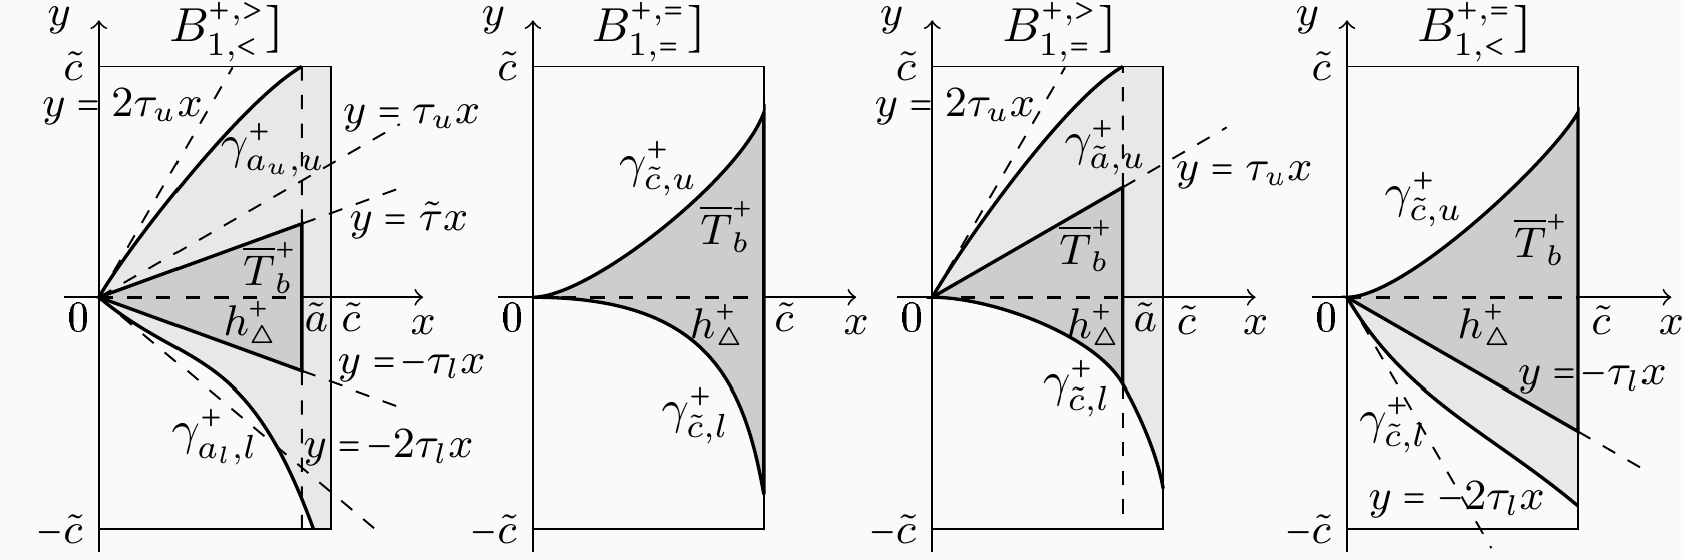
\includegraphics[width=0.9\textwidth]{boundary_curves_5}
    \end{figure}
\end{enumerate}

\subsection{Теоремы о существовании или отстутствии решений ГЗК}

\begin{theorem}[о существовании решения граничной задачи Коши]\label{th:ex:bound:1}
    Предположим, что в уравнении \eref{1.12} функция $ f_0 $ определена и непрерывна на множестве $ \vawe{G} $. \\
    Тогда в каждом из случаев $ (N_1^+), (U_1^{+, >}), (O_{1, <}^+), (B_{1, <}^{+, >}) $ и в каждом из случаев $ (U_1^{+, =}), (O_{1, =}^+) $, $ (B_{1, =}^{+, =}) $, $ (B_{1, =}^{+, >}), (B_{1, <}^{+, =}) $ при условиях \eref{1.15+} на любом правом граничном отрезке Пеано существует по крайней мере одно решение граничной задачи Коши с начальными данными $ (0, 0) $
\end{theorem}

\begin{proof}
    Рассмотрим, например, случай $ (B_{1, =}^{+, >}) $ \\
    Согласно \eref{1.13+} \nimp[(первые два неравенства)] правая верхнеграничная функция $ b_{a, u}^+(x) $, параметризующая кривую $ \gamma_{a_u, u}^+{}'(x) \ge \tau_u $ для любого $ x \in (0, a_u] $. А у правой нижнеграничной привой $ \gamma_{a_l, l}^+ $ константа $ a_l = c_O $ в силу \eref{1.13+} \nimp[(последние два нераенства)] \\
    Пусть $ c_* \define \min\set{c_U, c_O} $, тогда множество $ B_{c_*}^+ \setminus \big( \gamma_{a_u, u}^+ \cup \gamma_{a_l, l}^+ \big) \sub G $ \\
    Далее, для $ \tau_u $ найдётся (см. \eref{1.14}) такая $ \delta_{\tau_u} $, что $ |f_0(x, y)| \le \tau_u $ в любой точке $ \delta_{\tau_u} $-окрестности начала координат, принадлежащей $ \vawe{G} $ \\
    Положим $ \vawe{c} \define \min\set{c_*, \delta_{\tau_u}} $, тогда на множестве $ B_{\vawe{c}}^+ $ для функции $ |f_0| $ справедлива та же оценка \\
    Построим теперь лежащий в $ B_{\vawe{c}}^+ $ криволинейный треугольник $ \ol{T_b^+} $, как это было сделано при описании случая $ (B_{1, =}^{+, >}) $. Его высота $ h^+ = \vawe{a} $ \\
    Поскольку отрезок оси абсцисс $ [0, h^+] $ лежит в $ \vawe{G} $ и является отрезком поля направлений в точке $ O \in \hat{G} $, из точки $ O $ вправо можно начать строить ломаную Эйлера с проивольным рангом дробления \\
    Ломаная Эйлера не может покинуть $ \ol{T_b^+} $ через верхнюю боковую сторону, лежащую на прямой $ y = \tau_ux $, так как в любой её точке $ |f_0(x, y)| \le \tau_u $. Аналогично при попадании ломаной Эйлера при $ x = x_* > 0 $ на нижнюю боковую сторону, являющуюся частью правой нижнеграничной кривой $ \gamma_{\vawe{a}, l}^+ $, по условию \eref{1.15+} \nimp[(второе неравенство)] $ f_0 \big( x_*, b_{\vawe{a}, l}^+(x_*) \big) \ge b_{\vawe{a}}^+{}'(x_*) $, а значит, при $ x > x_* $ следующий отрезок ломаной будет либо лежать на $ \gamma_{\vawe{a}, l}^+ $, либо внутри треугольника в силу выпуклости $ \gamma_{\vawe{a}, l}^+ $. Поэтому ломаная Эйлера с произвольным выбранным рангом дробления может быть продолжена на весь правный граничный отрезок Пеано $ [0, h^+] $ \\
    Дальше дословно повторяется доказательство теоремы Пеано (теор. \ref{th:Peano}) \\
    Аналогичные рассуждения проводятся и в остальных случаях
\end{proof}

Рассмотренные в теореме \ref{th:ex:bound:1} девять случаев не исчерпывают все ситуации, в которых можно доказать существование решения ГЗК уравнения \eref{1.12}. Это удаётся сделать ещё в ряде случаев, но уже другим методом. \\
Все новые случаи предполагают наличие двух граничных функций, которые будем обозначать $ b_a^{+, u} $ и $ b_a^{+, l} $, а их графики -- $ \gamma_a^{+, u} $ и $ \gamma_a^{+, l} $. Например, $ \gamma_{a, u}^{+, l} $ -- это нижняя верхнеграничная кривая. При этом в определении граничных функций можно отказаться от условия о выпуклости, требуя от них только отсутсвия общих точек, кроме точки $ O $ \\
Для функций $ b_a^{+, *}(x) $ ($ * $ -- это $ u $ или $ l $) положим $ \tau^* \define \displaystyle{\half[b_a^{+, *}{}'(0)]} $ \\
Будем использовать два варианта сравнительного поведения правых граничных функций $ b_a^{+, *}{}'(x) $ и функции $ f_0(x, b_a^{+, *}) $ на отрезке $ [0, a] $:
\begin{equ}{1.16+}
    \begin{vars}
        f_0 \big( x, b_a^{+, u}(x) \big) \le b_a^{+, u}{}'(x), \quad f_0 \big( x, b_a^{+, l}(x) \big) \le b_a^{+, l}{}'(x) \\
        f_0 \big( x, b_a^{+, u}(x) \big) \ge b_a^{+, u}{}'(x), \quad f_0 \big( x, b_a^{+, l}(x) \big) \ge b_a^{+, l}{}'(x), \quad \tau^u \cdot \tau^l = 0
    \end{vars}
\end{equ}
Иными словами, в первом варианте построенные на обеих границах отрезки поля направлений напрвалены (с увеличением $ x $) по границе или внутрь области $ G $, лежащей между граничными кривыми, а во втором варианте -- наружу. Кроме того, во втором варианте требуется, чтобы хотя бы одна граничных кривых имела в начале координат горизонтальную касательную

\begin{theorem}[о существовании решения граничной задачи Коши]
    Пусть в уравнении \eref{1.12} функция $ f_0 $ определена и непрерывна на множестве $ \vawe{G} $ и имеет место один из вариантов из условия \eref{1.16+}, тогда на отрезке $ [0, a] $ существует по крайней мере одно решение ГЗК(0, 0)
\end{theorem}

\begin{proof}
	Без доказательства
\end{proof}

Перечислим и опишем новые случаи в привычных обозначениях: \\
Во-первых, ими являются три знакомых случая $ (B_{1, =}^{+, =}) $, $ (B_{1, =}^{+, >}) $, $ (B_{1, <}^{+, =}) $, но с иным поведением отрезков поля направлений на граничных кривых \\
Следующие два случая -- подслучаи $ (U_2^{+, =}) $, где стало существенно наличие второй верхнеграничной кривой и расположение области $ G $ между кривыми. Обозначим их $ (B_2^{+, >, =}) $, $ (B_2^{+, =, =}) $ по аналогии со случаем $ (B_{1, =}^{+, =}) $ \\
Последние два случая, обозначаемые $ (B_{2, =, =}^+) $ и $ (B_{2, <, =}^+) $ относятся к $ (O_{2, =}^+) $

\begin{figure}[!ht]
	\centering
    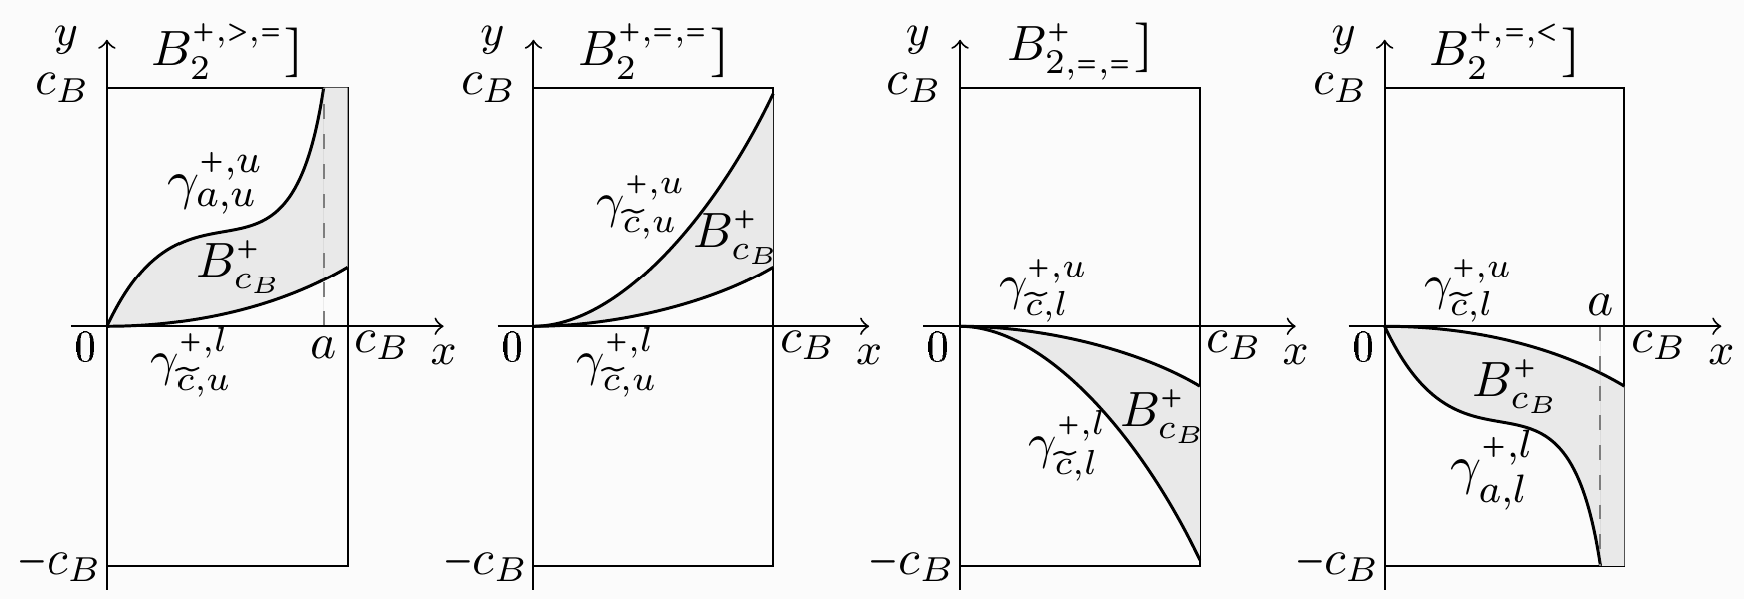
\includegraphics[width=0.95\textwidth]{boundary_curves_6}
\end{figure}

Изучим теперь нигде пока не рассмотренные случаи $ (U_2^{+, >}) $, $ (O_{2, <}^+) $, $ (B_{2, <}^{+, >}) $ и вырожденный случай $ (N_2^+) $: $ \exist c > 0 : \quad G \cap N_c^+ = \O $, в котором отсутсвуют граничные кривые, имеющие в точке $ O $ горизонтальную касательную:

\begin{theorem}[об отсутствии решений граничной задачи Коши]
    В каждом из случаев $ (U_2^{+, >}) $, $ (O_{2, <}^+) $, $ (B_{2, <}^{+, >}) $, $ (N_2^+) $ граничная задача Коши с начальными данными $ (0, 0) $ не имеет решений в правой полуплоскости
\end{theorem}

\begin{proof}
    Допустим, что в каждом случае из условия теоремы на некотором отрезке $ [0, a] $ существует решение $ y = \vphi(x) $ задачи Коши уравнения \eref{1.12} с начальными данными $ (0, 0) $, т. е. $ \vphi(0) = 0 $. Тогда $ \vphi'(0) = f_0 \big( 0, \vphi(0) \big) = 0 $. Но график любого решения должен лежать в $ \vawe{G} $, а значит, располагаться не ниже правой верхнеграничной кривой, у которой в точке $ O $ тангенс угла наклона согласно \eref{1.13+} равен $ 2\tau_u > 0 $, или не выше правой нижнеграничной кривой, имеющей в точке $ O $ тангенс угла наклона, равный $ -2\tau_l < 0 $. Поэтому $ \vphi'(0) \ne 0 $ -- \contra
\end{proof}

\begin{remark}
	Теоремы, подобные приведённым, можно сформулировать для левой полуплоскости
\end{remark}

\section{Единственность решения задачи Коши}

\subsection{Теорема о локальной единственности решения внутренней задачи Коши}

В этом разделе будет доказана теорема \ref{th:uniq-and-local-uniq} (о локальной единственности решения внутренней задачи Коши)

\begin{lemma}[о продолжимости решений на отрезок Пеано]
    Пусть $ y = \vphi(x) $ -- это решение внутренней задачи Коши с начальными данными $ x_0, y_0 $, определённое на $ \ol{P_h}(x_0, y_0) $. \\
    Тогда любое другое решение уравнения \eref{1.1} $ y = \psi(x) $ этой же задачи Коши, определённое на промежутке $ \braket{a, b} \subsetneq [x_0 - h, x_0 + h] $, продолжимо на $ \ol{P_h}(x_0, y_0) $
\end{lemma}

\begin{proof}
	Докажем, например, продолжимость решения $ y = \psi(x) $ с $ \psi(x_0) = y_0 $ на правый полуотрезок Пеано: \\
    Если $ \braket{a, b} = \langle a, b) $ (т. е. $ b \le x_0 + h $), то график решения $ y = \psi(x) $ при $ x \in [x_0, b) $ лежит в треугольнике $ \ol{T^+} $, построенном для решения $ y = \vphi(x) $. Поэтому у любой последовательности $ x_k \in [x_0, b) $ и $ x_k \infarr{k} b $ точки $ \big( x+k, \psi(x_k) \big) \in \ol{T^+} \sub \ol{R} $, а значит, найдётся сходящаяся последовательность $ \big( x_{k_l}, \psi(x_{k_l}) \big) $. Её предел -- точка $ (b, \eta) \in \ol{T^+} $ \\
    Следовательно, по теореме о продолжимости решения (теор. \ref{th:cont}) $ y = \psi(x) $ продолжимо на $ [x_0, b] $, хотя могло быть там сразу и задано
    \begin{itemize}
        \item Если теперь $ b = x_0 + h $, то лемма доказана
        \item Пусть $ b < x_0 + h $. Построим равнобедренный треугольник $ \ol{T_1^+} $ с вершиной в точке $ (b, \eta) $, боковыми сторонами, имеющими тангенсы углов наклона $ \pm M $, и основанием, лежащим на основании треугольника $ \ol{T^+} $ с абсциссой $ x_0 + h $. Тогда $ \ol{T_1^+} \sub \ol{T^+} $ и по теореме Пеано (теор. \ref{th:Peano}) на $ [b, x_0 + h] $ существует решение задачи Коши с начальными данными $ (b, \eta) $, продолжающее $ \psi(x) $ до точки $ x_0 + h $ включительно
    \end{itemize}
\end{proof}

По лемме для любой точки $ (x_0, y_0) \in G $ и для любого $ \ol{P_h}(x_0, y_0) $ любое решение задачи Коши уравнения \eref{1.1} с начальными данными $ x_0, y_0 $ продолжимо на $ [x_0 - h, x_0 + h] $. Поэтому, НУО будем считать, что все решения поставленной ЗК определены на выбранном отрезке $ \ol{P_h}(x_0, y_0) $. В частности, в определении локальной единственности решения (опр. \ref{def:uniq:local}) в качестве $ (\alpha, \beta) $ можно будет выбрать любой интервал из $ \ol{P_h}(x_0, y_0) $ \\
Пусть $ (x_0, y_0) \in G, \quad \ol{P_h}(x_0, y_0) $ -- некий отрезок Пеано и $ \seq{\chi_k(x)}k $ -- произвольная последовательность решений ЗК($ x_0, y_0 $) уравнения \eref{1.1}, определённых на $ [x_0 - h, x_0 + h] $

\begin{statement}\label{st:2}
	Для любых $ k \in \N, \quad x \in [x_0 - h, x_0 + h] $ функции
    $$ \chi_k^l(x) \define \min\set{\chi_1(x), ..., \chi_k(x)}, \qquad \chi_k^u(x) \define \max\set{\chi_1(x), ..., \chi_k(x)} $$
    также являются решениями поставленной задачи на $ \ol{P_h}(x_0, y_0) $
\end{statement}

\begin{proof}
    Действительно, эти функции удовлетворяют всем трём условиям из определения решения, поскольку для любого $ x_* \in [x_0 - h, x_0 + h] $ найдётся такой индекс $ 1 \le \bm{j} \le k $, что, например, $ \chi_k^l(x_*) = \chi_j(x_*) $, и если $ \chi_j(x_*) = \chi_m(x_*) $, то $ \chi_j'(x_*) = \chi_m'(x_*) = f \big( x_*, \chi_k^l(x_*) \big) $
\end{proof}

\begin{lemma}[о нижнем и верхнем решениях]
    Существуют решения ЗК($ x_0, y_0 $) $ y = \chi^l(x) $ и $ y = \chi^u(x) $ уравнения \eref{1.1} такие, что
    \begin{equ}{1.19}
    	\forall k \in \N \quad \forall x \in [x_0 - h, x_0 + h] : \quad
        \begin{cases}
        	\chi^l(x) \le \chi_k^l(x) \\
            \chi^u(x) \ge \chi_k^u(x)
        \end{cases}
    \end{equ}
\end{lemma}

\begin{proof}
    Рассмотрим, например, последовательность решений $ \seq{x_k^l(x)}k $ на отрезке \\
    $ [x_0, x_0 + h] $. Поскольку все их графики лежат в треугольнике $ \ol{T^+} $, полученном при построении отрезка Пеано, эта последовательность равномерно ограничена и равностепенно ограничена (см. док-во теоремы Пеано). Следовательно, по лемме Арцела-Асколи из неё можно выделить равномерно на $ \ol{P_h}{(x_0, y_0)} $ сходящуюся подпоследовательность, предел которой тоже будет решением уравнения \eref{1.1} на отрезке Пеано \\
    Но последовательность $ \chi_k^l(x) $ монотонно убывает, поэтому она сама будет сходиться к нижнему решению $ y = \chi^l(x) $, для которого, очевидно, будет верно неравенство \eref{1.19} \\
    Рассуждения для отрезка аналогичны так же, как и доказательство сходиомости функции $ \chi_k^u(x) $ к верхнему решению $ y = \chi^u(x) $
\end{proof}

\begin{theorem}[о локальной единственности решения внутренней ЗК]
	Пусть $ (x_0, y_0) \in G $ -- это точка единственности. \\
    Тогда решение ЗК($ x_0, y_0 $) уравнения \eref{1.1} является локально единственным
\end{theorem}

\begin{proof}
    \bt{От противного} \\
    Построим какой-нибудь отрезок Пеано $ \ol{P_h(x_0, y_0)} $ и допустим, что для любого интревала $ (\alpha, \beta) $ такого, что $ x_0 \in (\alpha, \beta) \sub [x_0 - h, x_0 + h] $, существуют такие решения ЗК $ y = \vphi(x) $ и $ y = \psi(x) $, не совпадающие на $ (\alpha, \beta) $ \\
    Тогда для всякого $ k = 1, 2, ... $ найдутся решения $ y = \vphi_k(x) $ и $ y = \psi_k(x) $ ЗК, определённые на отрезке Пеано, такие, что
    $$ \exist x_k \in \bigg( x_0 - \frac{h}k, x_0 + \frac{h}k \bigg) : \quad \vphi_k(x_k) < \psi_k(x_k) $$
    Согласно утверждению \ref{st:2} функция $ \vphi_k^l = \min\set{\vphi_1(x), ..., \vphi_k(x)} $ и функция $ \psi_k^u(x) $, удовлетворяющие неравенства типа \eref{1.19} \\
    В результате $ x_k \infarr{k} x_0 $ и справедливы неравенства
    $$ \forall k = 1, 2, ... \quad \vphi^l(x_k) \le \vphi_k(x_k) < \psi_k(x_k) \le \psi^u(x_k) $$
    означающие, что $ (x_0, y_0) $ -- точка единственности -- \contra
\end{proof}

\subsection{Лемма Гронуолла}

\begin{lemma}[Гронуолла; об интегральной оценке функции сверху]\label{lm:Gron}
    Пусть функция $ h(x) \in \Cont{\braket{a, b}} $ и существуют такие $ x_0 \in \braket{a, b}, \quad \lambda \ge 0, \quad \mu > 0 $, что
    \begin{equ}{1.20}
        \forall x \in \braket{a, b} \quad 0 \le h(x) \le \lambda + \mu \bigg| \dint[s]{x_0}x{h(s)} \bigg|
    \end{equ}
    Тогда для любого $ x \in \braket{a, b} $ справедливо неравенство
    \begin{equ}{1.21}
        h(x) \le \lambda e^{\mu|x - x_0|}
    \end{equ}
\end{lemma}

\begin{iproof}
	\item Предположим, что $ x \ge x_0 $ \\
    Введём в рассмотрение функцию $ g(x) = \dint[s]{x_0}x{h(s)} $
    $$ \implies \quad g(x_0) = 0, \qquad g(x) \ge 0, \qquad g(x) \in \Cont[1]{[x_0, b \rangle}, \qquad g'(x) = h(x) \ge 0 $$
    Подставим $ g(x) $ в \eref{1.20}:
    $$ g'(x) \le \lambda + \mu g(x) \quad \implies \quad g'(x) - \mu g(x) \le \lambda \quad \implies \quad e^{-\mu(x - x_0)} \bigg( g'(x) - \mu g(x) \bigg) \le \lambda e^{-\mu(x - x_0)} $$
    При этом,
    $$ \bigg( g(x) e^{-\mu(x - x_0)} \bigg)' = g'(x)e^{-\mu(x - x_0)} - \mu e^{-\mu(x - x_0)} g(x) = e^{-\mu(x - x_0)} \bigg( g'(x) - \mu g(x) \bigg) $$
    Отсюда
    $$ \bigg( g(x) e^{-\mu(x - x_0)} \bigg)' \le \lambda $$
    Проинтегрируем по $ s $ от $ x_0 $ до $ x $:
    $$ g(x)e^{-\mu(x - x_0)} - \underbrace{g(x_0)}_0 \le \lambda \dint[s]{x_0}x{e^{-\mu(s - x_0)}} = -\frac\lambda\mu(e^{-\mu(x - x_0)} - 1) $$
    Умножим на $ e^{\mu(x - x_0)} $:
    $$ g(x) \le \frac\lambda\mu (e^{\mu(x - x_0)} - 1) $$
    Подставим в \eref{1.20}:
    $$ h(x) \le \lambda + \mu g(x) \le \lambda e^{\mu(x - x_0)} $$
    Таким образом, неравенство доказано для всех $ x \in [x_0, b \rangle $
    \item Если $ x \le x_0 $, то в \eref{1.20}
    $$ h(x) \le \lambda - \mu \dint[s]{x_0}x{h(s)}, \qquad g(x) \le 0 $$
    Дальнейшее доказательство аналогично
\end{iproof}

\begin{implication}
	Если $ \lambda = 0 $, то есть
    $$ 0 \le h(x) \le \mu \bigg| \dint[s]{x_0}x{h(s)} \bigg| $$
    то $ h(x) \overset{\braket{a, b}}\equiv 0 $
\end{implication}

\subsection{Условия Липшица}

Бывает, что требование дифференцируемости функции оказывается чрезмерным. Тогда его заменяют ``локальным условием Липшица'', которое не допускает более чем линейного роста функции по этой переменной в малой окрестности каждой точки из некоторого множества

\begin{definition}
	Функция $ f(x, y) $ удовлетворяет условию Липшица по $ y $ глобально на множестве $ D \sub \R^2 $, если
    \begin{equ}{1.22}
        \exist L > 0 : \quad \forall (x, y_1), (x, y_2) \in D \quad |f(x, y_1) - f(x, y_2)| \le L|y_1 - y_2|
    \end{equ}
\end{definition}

\begin{notation}
    $ f \in \operatorname{Lip}_y^{gl}(D) $
\end{notation}

\begin{definition}
    Функция $ f(x, y) $ удовлетворяет условию Липшица по $ y $ локально на множестве $ \vawe{G} $, если для любой точки $ (x_0, y_0) \in \vawe{G} $ найдётся замкнутая $ c $-окрестность $ \ol{B}_c(x_0, y_0) $ такая, что функция $ f $ удовлетворяет условию Липшица по $ y $ глобально на множестве $ U_c = \vawe{G} \cap \vawe{B}_c(x_0, y_0) $
\end{definition}

\begin{notation}
    $ y \in \operatorname{Lip}_y^{loc}(\vawe{G}) $
\end{notation}

\subsection{Теоремы о глобальной единственности решений}

\begin{theorem}[о множестве единственности]
    Пусть в уравнении \eref{1.1} функция $ f(x, y) $ опредлена и непрерывна на множестве $ \vawe{G} $ и удовлетворяет условию Липшица по $ y $ локально на множестве $ \vawe{G^0} = G^0 \cup \hat{G^0} $, \nimp[где $ G^0 \sub G $ -- область, а $ \hat{G^0} \sub \partial G^0 \cap \hat{G} $]. \\
    Тогда $ \vawe{G^0} $ -- множество единственности для уравнения \eref{1.1}
\end{theorem}

\begin{proof}
    Возьмём любую точку $ (x_0, y_0) $ из множества $ \vawe{G^0} $ и покажем, что она является точкой единственности. \\
    Поскольку $ f \in \operatorname{Lip}_y^{loc}(\vawe{G^0}) $, найдутся $ \ol{B}_c(x_0, y_0) $ и $ L > 0 $ такие, что $ f \in \operatorname{Lip}_y^{gl}(U_c) $ с константой $ L $, где $ U_c = \vawe{G^0} \cap \ol{B}_c(x_0, y_0) $
    \begin{itemize}
        \item Если $ (x_0, y_0) \in G^0 $, то найдётся $ c > 0 $ такое, что $ U_c = \ol{B}_c(x_0, y_0) $, решение ЗК($ x_0, y_0 $) существует на некотором интервале $ (a, b) \ni x_0 $ и для любого решения этой задачи, уменьшая при необходимости $ (a, b) $, можно добиться, чтобы его график лежал в $ U_c $
        \item Пусть $ (x_0, y_0) \in \hat{G^0} $
        \begin{itemize}
            \item Если решение ЗК($ x_0, y_0 $) отсутсвует, то $ (x_0, y_0) $ -- это точка единственности по определению
            \item Пусть решение существует на некотром промежутке $ \braket{a, b} $ таком, что $ x_0 \in \braket{a, b} \sub [x_0 - c, x_0 + c] $
            \begin{statement}
                Тогда, уменьшая $ \braket{a, b} $ при необходиости можно добиться, чтобы график решения лежал в $ U_c $
            \end{statement}
            \begin{proof}
                Действительно, очевидно, что с уменьшением $ \braket{a, b} $ график решения попадает в $ \ol{B}_c(x_0, y_0) $. А ситуация, когда при $ x < x_0 $ и (или) $ x > x_0 $ график, оставаясь в $ \vawe{G} $, не принадлежит $ \vawe{G^0} $, преодолевается за счёт выбора константы $ c_1 > c $ такой, что в $ \ol{B}_{c_1}(x_0, y_0) $ юудет выполняться глобальное условие Липшица с константой, скажем, $ L_1 \define L + 1 $. В результате с учётом непрерывности функции $ f(x, y) $ бласть $ \vawe{G^0} $ увеличиться, включив в себя дугу интегральной кривой в малой окрестности точки $ (x_0, y_0) $
            \end{proof}
        \end{itemize}
    \end{itemize}
    Рассмотрим любые два решения $ y = \vphi_1(x) $ и $ y = \vphi_2(x) $ ЗК($ x_0, y_0 $), которые определены по крайней мере на некотором общем промежутке $ \braket{\alpha, \beta} $ таком, что $ x_0 \in \braket{\alpha, \beta} \sub [x_0 - c, x_0 + c] $ \\
    Как установлено выше, уменьшая при необходимости $ \braket{\alpha, \beta} $, можно добиться, чтобы для всякого $ x \in \braket{\alpha, \beta} $ точки $ \big( x, \vphi_1(x) \big), \big( x, \vphi_2(x) \big) \in U_c $ \\
    По лемме о записи решения в интегральном виде $ \vphi_1(x) $ и $ \vphi_2(x) $ удовлетворяют тождеству \eref{1.2} на $ \braket{\alpha, \beta} $, т. е. для любого $ x \in \braket{\alpha, \beta} $ справедливо
    $$ \vphi_j(x) = \vphi_j(x_0) + \dint[s]{x_0}x{f \big( s, \vphi_j(s) \big)}, \qquad j = 1, 2 $$
    Поэтому
    $$ \vphi_2(x) - \vphi_1(x) = \dint[s]{x_0}x{\bigg( f \big( s, \vphi_2(s) \big) -  \big( s, \vphi_1(s) \big) \bigg)} $$
    точки $ \big( s, \vphi_j(s) \big) \in U_c $ и для них выполнено неравенство \eref{1.22}. Тогда
    $$ |\vphi_2(x) - \vphi_1(x)| \le \bigg| \dint[s]{x_0}x{\big| f \big( s, \vphi_2(s) \big) - f \big( s, \vphi_1(s) \big) \big|} \bigg| \le \bigg| \dint[s]{x_0}x{L \big| \vphi_2(s) - \vphi_1(s) \big|} \bigg| $$
    К последнему неравенству можно применить следствие к лемме Гронуолла (лемма \ref{lm:Gron}), где $ h(x) = |\vphi_2(x) - \vphi_1(x)|, \quad \lambda = 0, \quad \mu = L $ \\
    Тогда $ |\vphi_2(x) - \vphi_1(x)| \overset{\braket{\alpha, \beta}}\equiv 0 $, т. е. решения $ y = \vphi_1(x) $ и $ \vphi_2(x) $ ЗК($ x_0, y_0 $) совпадают в каждой точке $ \braket{\alpha, \beta} \ni x_0 $. Поэтому по определению $ (x_0, y_0) $ -- это точка единственности
\end{proof}

\begin{undefthm}{Частный случай}
    Предположим, что в уравнении \eref{1.1} функция $ f(x, y) $ непрерывна в области $ G $ и удовлетворяет условию Липшица по $ y $ локально в области $ G^0 \sub G $. \\
    Тогда $ G^0 $ -- это область единственности
\end{undefthm}

\begin{theorem}[о множестве единственности; слабая]
    Предположим, что в уравнении \eref{1.1} функция $ f(x, y) $ определена и непрерывна на множестве $ \vawe{G} $, функция $ \pder{f(x, y)}y $ определена и непрерывна в области $ G^0 \sub G $. \\
    Тогда мноежство $ \vawe{G^0} = G^0 \cup \hat{G^0} $, \nimp[где $ \hat{G^0} \sub \partial G^0 \cap \hat{G} $ и состоит из точек, в которых $ \pder{f(x, y)}y $ может быть доопределена по непрерывности], является множеством единственности для уравнения \eref{1.1}, если при этом для любой точки $ (x_0, y_0) \in \hat{G^0} $ найдётся $ \ol{B}_c(x_0, y_0) $ такая, что множество $ \vawe{G^0} \cap \ol{B}_c(x_0, y_0) $ выпукло по $ y $
\end{theorem}

\begin{note}
	Выпуклость множетсва по $ y $ означает, что множеству принадлежит отрезок, соединяющий любые две его точки с одинаковой абсциссой
\end{note}

\begin{note}
    Существование функции $ \pder{f(x, y)}y $ предполагается только в области, а на границе её приходится доопределять, поскольку для определения частной производной обычно требуется, чтобы функция $ f $ была задана в полной окрестности этой точки
\end{note}

\begin{note}
    В последнем пердположении теоремы говорится о произвольной точке границы множества $ \vawe{G^0} $, поскольку для любой точки из области $ G^0 $ требуемое условие выполняется автоматически
\end{note}

\begin{proof}
    Рассмотрим произвольную точку $ (x_0, y_0) \in \vawe{G^0} $. Поскольку функция $ \pder{f(x, y)}y $ непрерывна в точке $ (x_0, y_0) $, существует такое $ \delta $, что $ 0 \le \delta \le c $, где  $ c $ берётся из формулировки теоремы, и для любой точки $ (x, y) \in U_\delta \define \vawe{G^0} \cap \ol{B}_\delta(x_0, y_0) $ верно неравенство
    $$ \bigg| \pder{f(x, y)}y - \pder{f(x_0, y_0)}y \bigg| \le 1 $$
    Таким образом, установлено, что $ U_\delta $ выпукло по $ y $ и
    $$ \bigg| \pder{f(x, y)}y \bigg| \le L \define \bigg| \pder{f(x_0, y_0)}y \bigg| + 1 \quad \forall (x, y) \in U_\delta $$
    По теореме Лагранжа для любых двух точек $ (x, y_1), (x< y_2) \in U_\delta, \quad y_1 < y_2 $,
    $$ \exist y^*(x) \in (y_1, y_2) : \quad f(x, y_2) - f(x, y_1) = \pder{f \big( x, y*(x) \big)}y(y_2 - y_1) $$
    Здесь точка $ \big( x, y^*(x) \big) \in U_\delta $, так как множество $ U_\delta $ выпукло по $ y $. Поэтому в $ U_\delta $ верно неравенство
    $$ |f(x, y_2) - f(x, y_1)| \le L|y_2 - y_1| $$
    означающее, что $ f \in \operatorname{Lip}_y^{gl}(U_\delta) $. Тогда по определению выполнено локальное условие Липшица, а значит, по теореме о единственности $ \vawe{G^0} $ -- это множество единственности
\end{proof}

Не только гладкость функции $ f $ по $ y $, но и локальное условие Липшица не является необходимым:

\begin{theorem}[Осгуда; о единственности в области; сильная]
    Пусть в уравнении \eref{1.1} функция $ f(x, y) $ непрерывна в области $ G $ и
    \begin{equ}{1.24}
    	\foral (x, y_1), (x, y_2) \in G \quad |f(x, y_2) - f(x, y_1)| \le h \big( |y_2 - y_1| \big)
    \end{equ}
    где функция $ h(s) $ определена, непрерывна и положительна для всякого $ s \in (0, +\infty) $ и
    $$ \dint[s]\veps{a}{h^{-1}(s)} \underarr{\veps \to 0} \infty, \qquad a > \veps > 0 $$
    Тогда $ G $ -- это область единственности для уравнения \eref{1.1}
\end{theorem}

\begin{proof}
	Без доказательства
\end{proof}

\begin{remark}
    В качаестве $ h(s) $ можно выбрать линейную функцию $ Ls $. Тогда неравенство \eref{1.24} окажется глобальным условием Липшица, а теорема о единственности будет вытекать из теоремы Осгуда
\end{remark}

\section{Существование общего решения}

В этом параграфе будет доказана теорема о существовании общего решения (теор. \ref{th:comm:exist})

\subsection{Область существования общего решения}

Опишем множество $ A^* $, в котором можно построить общее решение, поскольку гарантировать его существование во всей области единственности $ G^0 $ нельзя, какой бы малой она ни была \\
В этом параграфе в роли $ A^* $ будет выступать вводимый ниже компакт $ \ol{A} $

\begin{algorithm}[построения $ \ol{A} $]
    Пусть $ G^0 $ -- область единственности для уравнения \eref{1.1} \\
    Возьмём любую точку $ (x_0^*, y_0^*) \in G^0 $ \\
    Поскольку $ G^0 $ является открытым множеством, существует такое $ \delta > 0 $, что $ \ol{B}_{2\delta}(x_0^*, y_0^*) \sub G^0 $ \\
    Пусть числа $ y_1, y_2 $ таковы, что
    $$
    \begin{cases}
    	0 < y_0^* - y_1 < \delta \\
        0 < y_2 - y_0^* < \delta
    \end{cases} $$
    и найдётся отрезок $ [a, b] \ni x_0^* $ такой, что графики решений ЗК($ x_0^*, y_1 $) $ y = \vphi_1(x) $ и ЗК($ x_0^*, y_2 $) $ y = \vphi_2(x) $ лежат в $ \ol{B}_c $ при $ x \in [a, b] $. Тогда в $ \ol{B}_\delta $ содержится компакт
    \begin{equ}{1.25}
        \ol{A} = \set{(x, y) | a \le x \le b, \quad \vphi_1(x) \le y \le \vphi_2(x)}
    \end{equ}
\end{algorithm}

При этом $ A $ \nimp[(то же самое, со строгими неравенствами)] -- это область, так как по построению $ \vphi_1(x_0^*) = y_1 < y_2 = \vphi_2(x_0^*) $, а значит, $ \vphi_1(x) < \vphi_2(x) $ для всякого $ x \in [a, b] $, поскольку в области единственности $ G^0 $ дуги интегральных кривых не могут соприкасаться и разбивать $ A $ на несвязные подмножества

\begin{lemma}[о поведении решений на компакте $ \ol{A} $]\label{lm:comp}
    Для любой точки $ (x_0, y_0) \in \ol{A} $ решение \caupr[\eref{1.1}]{x_0, y_0} $ y = \vphi(x) $ продолжимо на отрезок $ [a, b] $
\end{lemma}

\begin{proof}
    Для любой точки $ (x_0^*, y_0^*) \in G^0 $ построим компакт $ \ol{A} $ вида \eref{1.25}, тогда $ \ol{A} \sub \ol{B}_\delta \sub \ol{B}_{2\delta} \sub G^0 $ \\
    Возьмём произвольную точку $ (x_0, y_0) \in \ol{A} $. Тогда прямоугольник
    $$ \ol{R} \define \set{(x, y) | {} |x - x_0| \le \delta, \quad | y - y_0| \le \delta} \quad \sub \ol{B}_{2\delta} $$
    Пусть $ M \define \max_{\ol{B}_{2\delta}}|f(x, y)| > 0 $ (при $ M = 0 $ лемма очевидна) \\
    Положим $ h \define \min\set{\delta, \faktor\delta{M}} $. Тогда $ P_h(x_0, y_0) = [x_0 - h, x_0 + h] $ -- отрезок Пеано, построенный для произвольной точки $ (x_0, y_0) \in \ol{A} $ \\
    Следовательно, по теореме Пеано решение \caupr{x_0, y_0} $ y = \vphi(x) $ определено на отрезке Пеано $ [x_0 - h, x_0 + h] $, длина которого неизменна для всех точек $ (x_0, y_0) \in \ol{A} $
    \begin{itemize}
    	\item Рассмотрим функцию $ \vphi(x) $ при $ x > x_0 $:
        \begin{itemize}
        	\item Если $ x_0 + h < b $, то $ \vphi_1(x_0 + h) \le \vphi(x_0 + h) \le \vphi_2(x_0 + h) $, а значит, точчка $ x_0 + h, \big( x_0 + h, \vphi(x_0 + h) \big) $ \\
            Выбрав эту точку в качетстве начальной, решение $ y - \vphi(x) $ можно продолжить вправо на полуотрезок Пеано $ [x_0 + h, x_0 - h] $
            \begin{itemize}
            	\item Если $ x_0 + 2h \ge b $, то лемма доказана
                \item Иначе сделаем очередное продолжение решения вправо на длину $ h $ \\
                В результате за конечное число шагов будет продолжено вправо до точки $ b $ включительно
            \end{itemize}
        \end{itemize}
        \item Аналогично $ y = \vphi(x) $ можно продолжить влево до точки $ a $
    \end{itemize}
\end{proof}

\subsection{Формула общего решения}

Для любой точки $ (x_0, y_0) \in \ol{A} $ обозначим через $ y = y(x, x_0, y_0) $ решение \caupr[\eref{1.1}]{x_0, y_0} \\
Тогда $ y(x_0, x_0, y_0) = y_0 $, и по лемме о поведении решений на компакте (лемма \ref{lm:comp}) решение $ y = (x, x_0, y_0) $ определено для всякого $ x \in [a, b] $ \\
Для произвольной точки $ \zeta \in [a, b] $ рассмотрим функцию
\begin{equ}{1.26}
    \vphi(x C) = y(x, \zeta, C), \qquad (\zeta, C) \in \ol{A}
\end{equ}
на прямоугольнике $ \ol{Q} = \ol{Q}_{\ol{A}} \define \set{(x, C) | a \le x \le b, \quad \vphi_1(\zeta) \le C \le \vphi_2(\zeta)} $, который является частным случаем множества $ Q_{A^*} $ из определения общего решения (опр. \ref{def:common}) \\
В самом деле, $ \vphi_1(\zeta) \le C \le \vphi_2(\zeta) $ по построению $ \ol{A} $. А по лемме решение $ y = y(x, \zeta, C) $ определено для любого $ x \in [a, b] $ и при $ x = \zeta $ по определению решения ЗК $ \vphi(\zeta, C) = y(\zeta, \zeta, C) = C $

\begin{theorem}[о существовании общего решения]
    Введённая в формуле \eref{1.26} функция $ y = \vphi(x, C) $ является общим решением уравнения \eref{1.1} на компакте $ \ol{A} $ из \eref{1.25}, построенном в окрестности произвольной точки из области единственности $ G^0 $
\end{theorem}

\begin{proof}
    Покажем, что функция $ y = \vphi(x, C) $ удовлетворяет определению общего решения уравнения \eref{1.1}:
    \begin{enumerate}
        \item Возьмём произвольную точку $ (x_0, y_0) \in \ol{A} $ и рассмотрим уравнение $ y_0 = \vphi(x_0, C) $ или согласно \eref{1.26} уравнение
        \begin{equ}{1.27}
        	y_0 = y(x_0, \zeta, C)
        \end{equ}
        Наличие у него решения $ C = C_0 $ фактически означает, что ``выпущенное'' из точки $ (\zeta, C_0) \in \ol{A} $ решение уравнения \eref{1.1} в момент $ x_0 $ попадает в точку $ (x_0, y_0) \in \ol{A} $ \\
        Покажем, что решение уравнения \eref{1.27} сущетсувует и единственно: \\
        ``Выпустим'' из точки $ (x_0, y_0) $ решение $ y = y(x, x_0, y_0) $, которое по лемме \ref{lm:comp} определено на всём отрезке $ [a, b] $ и, в частности, при $ x = \zeta \in [a, b] $ по определению \eref{1.26} \\
        Пусть $ C_0 = y(\zeta, x_0, y_0) $. Тогда $ (\zeta, C) $ -- это точка единственности, так как принадлежит графику решения $ y = y(x, x_0, y_0) $ \\
        Поэтому решение \caupr{\zeta, C} $ y = u(x, \zeta, C_0) $ с начальными данными $ \zeta, C_0 $ по лемме о поведении решений на компакте $ \ol{A} $ (лемма \ref{lm:comp}) продолжимо на $ [a, b] $ и совпадает с решением $ y = y(x, x_0, y_0) $ \\
        Следовательно, $ y_0 = y(x_0, \zeta, C) $, т. е. график функции $ y = y(x, \zeta, C_0) $ проходит через точку $ (x_0, y_0) $. Другими словами, дуга интегральной кривой, проходящая через точки $ (x_0, y_0) $, $ (\zeta, C_0) $, имеет на отрезке $ [a, b] $ две параметризации $ y = y(x, x_0, y_0) $ и $ y = (x, \zeta, C_0) $ \\
        Итак, установлено, что уравнение \eref{1.27} имеет единственное решение $ C = C_0 = y(\zeta, x_0, y_0) $, т. е. $ y_0 = y \big( x_0, \zeta, y(\zeta, x_0, y_0) \big) $
        \item Функция $ y = \vphi(x, C_0) $ является решением \caupr[\eref{1.1}]{x_0, y_0}, поскольку согласно \eref{1.26} и \eref{1.27} $ \vphi(x_0, C_0) = y(x_0, \zeta, C_0) = y_0 $
        \item Осталось доказать, что функция $ y = \vphi(x, C) $ из \eref{1.26} непрерывна на компакте $ \ol{Q} $ по совокупности переменных:
        \begin{itemize}
        	\item Поскольку для всякого $ C \in [\vphi_1(\zeta), \vphi_2(\zeta)] $ функция $ y = \vphi(x, C) $ -- это решение уравнения \eref{1.1}, она непрерывна по $ x $ при $ x \in [a, b] $
            \item Покажем, что для всякого $ x \in [a, b] $ функция $ y = \vphi(x, C) $ непрерывна по $ C $ при $ C \in [\vphi_1(\zeta), \vphi_2(\zeta)] $: \\
            Допуская \bt{противное}, предположим, что найдутся $ \vawe\veps > 0 $, $ \vawe{x} \in [a, b] $ и последовательность $ C_k \infarr{k} \vawe{C} $, $ C_k \in [\vphi_1(\zeta), \vphi_2(\zeta)] $ такие, что $ \big| \vphi(\vawe{x}, C_k) - \vphi(\vawe{x}, \vawe{C}) \big| \ge \vawe\veps $ при всех $ k \ge 1 $. Это значит, что при $ x = \vawe{x} $ функция $ \vphi(\vawe{x}, C) $ терпит разрыв в точке $ \vawe{C} \in [\vphi_1(\zeta), \vphi_2(\zeta)] $, поскольку любой компакт, в частности отрезок $ [\vphi_1(\zeta), \vphi_2(\zeta)] $, содержит все свои предельные точки. В этом случае, кстати, $ \vawe{x} \ne \zeta $, так как по определению $ \vphi(\zeta, C_k) = C_k \infarr{k} C = \vphi(\zeta, C) $ \\
            Выпуская из точек $ (\zeta, C_k) \in \ol{A} $ дуги интегральных кривых, получаем последовательность решений $ y = y(x, \zeta, C_k) = \vphi(x, C_k) $. Поскольку из любой сходящейся последовательности можно выдулить монотонную подпоследовательность, НУО считаем, что последовательность $ C_k $ монотонно возрастает, т. е. $ C_k < C_{k + 1} < \vawe{C} $ для любого $ k \ge 1 $ \\
            В области $ G^0 $ интегральные кривые не имеют общих точек, поэтому последовательность $ \vphi(\vawe{x}, C_k) $ тоже монотонно возрастает и ограничена, так как $ \vphi(\vawe{x}, C_k) \le \vphi(\vawe{x}, \vawe{C}) - \vawe\veps $ по предположению. Но любая ограниченная монотонная последовательность имеет предел \\
            Пусть $ \vawe{y} = \limi{k} \vphi(\vawe{x}, C_k) $, тогда $ \vawe{y} \le \vphi(\vawe{x}, \vawe{C}) - \vawe\veps $ \\
            Выберем произвольную точку $ y^* $ из интервала $ \big( \vawe{y}, \vphi(\vawe{x}, \vawe{C}) \big) $ \\
            Рассмотрим определённое на $ [a, b] $ решение \caupr{\vawe{x}, y^*}, обозначаемое $ y = y(x, \vawe{x}, y^*) $ \\
            Пусть $ C^* = y(\zeta, \vawe{x}, y^*) $. Тогда $ C^* < \vawe{C} $, так как $ y^* < \vphi(\vawe{x}, \vawe{C}) = y(\vawe{y}, \zeta, \vawe{C}) $ \\
            Дугу интегральной кривой решения $ y = y(x, \vawe{x}, y^*) $ на $ [a, b] $, как было установлено, параметризует также решение с начальными данными $ \zeta, C^* $, имеющее согласно формуле \eref{1.26} вид $ y = \vphi(x, C^*) $, причём $ \vphi(\vawe{x}, C^*) = y^* $ \\
            Однако существует индекс $ k^* $ такой, что член $ C^{k*} $ сходящейся к $ \vawe{C} $ последовательности $ C_k $ будет больше, чем $ C^* $ \\
            В результате получилось так, что дуги интегральных кривых решений $ y = \vphi(x, C_{k*}) $ и $ y = \vphi(x, C^*) $ пересекаются в некоторой точке $ x^* $, лежащей между $ \zeta $ и $ \vawe{x} $, поскольку $ \vphi(\zeta, C_{k*}) = C_{k*} > C^* = \vphi(\zeta, C^*) $, а $ \vphi(\vawe{x}, C_{k*}) < \vawe{y} < y^* = y(\vawe{x}, \zeta, C^*) = \vphi(\vawe{x}, C^*) $ -- \contra с тем, что $ G $ -- область единственности
        \end{itemize}
        Итак, доказано, что функция $ y = \vphi(x, C) $ непрерывна по каждой из переменных в прямоугольнике $ \ol{Q} $. Но этого недостаточно для её непрерывности по совокупности переменных \\
        Воспользуемся ещё одним свойством функции $ \vphi $: \\
        Поскольку $ y = \vphi(x, C) $ при любой константе $ C \in [\vphi_1(\zeta), \vphi_2(\zeta)] $ есть решение уравнения \eref{1.1}, то $ \pder{\vphi(x, C)}x \equiv f \big( x, \vphi(x, C) \big) $ на $ [a, b] $ \\
        Но $ \big( x, \vphi(x, C) \big) \in \ol{A} $, когда точка $ (x, C) \in \ol{Q} $, а на компакте $ \ol{A} $ выполняется неравенство $ |f(x, y)| \le M $. Следовательно, функция $ \big| \pder{\vphi(x, C)}x \big| $ ограничена на $ [a, b] $ \\
        С учётом теоремы Лагранжа заключаем, что для любой константы $ C \in [\vphi_1(\zeta), \vphi(\zeta)] $ и для любых $ x_1, x_2 \in [a, b], ~ x_1 < x_2 $ найдётся такое $ x_C \in (x_1, x_2) $, что $ \vphi(x_2, C) - \vphi(x_1, C) = \pder{\vphi(x_C, C)}x(x_2 - x_1) $ \\
        Этого достаточно, чтобы непрерывность функции $ y = \vphi(x, C) $ по $ x $ на $ [a, b] $, равномерная относительно $ C \in [\vphi_1(\zeta), \vphi_2(\zeta)] $ в силу признака Вейрештрасса с $ \delta = \faktor\veps{M} $, стала очевидной \\
        Последнее свойство функции $ \vphi $ наряду с её поточечной непрерывностью по $ C $ гранатирует непрерывность $ \vphi(x, C) $ по совокупности переменных в прямоугольнике $ \ol{Q} $ \\
        Действительно, возьмём произвольную точку $ (x_0, C_0) \in \ol{Q} $ и покажем, что функция $ \vphi(x, C) $ непрерывна в этой точке: \\
        Для этого зафиксируем любое число $ \veps > 0 $. Тогда в силу непрерывности функции $ \vphi $ по $ C $ найдётся такое $ \delta_{x_0} > 0 $, что
        $$ \foral C \quad \nimp[\bigg(] |C - C_0| < \delta_{x_0} \implies |\vphi(x_0, C) - \vphi(x_0, C_0)| < \half[\veps] \nimp[\bigg)] $$
        А из равномерной непреывности $ \vphi(x, C) $ по $ x $ относительно $ C $ вытекает, что
        $$ \exist \delta_0 > 0 : \quad \foral C \in [x\vphi_1(\zeta), \vphi_2(\zeta)] \quad \forall x \quad \nimp[\bigg(] |x - x_0| < \delta_0 \implies |\vphi(x, C) - \vphi(x_0, C)| < \half[\veps] \nimp[\bigg)] $$
        Выберем число $ \delta \define \min\set{\delta_{x_0}, \delta_0} $, тогда для любой точки $ (x, C) $ получаем:
        $$ \norm{(x, C) - (x_0, C_0)} \define \max\set{|x - x_0|, |C - C_0|} < \delta $$
        Следовательно,
        $$ |\vphi(x, C) - \vphi(x_0, C_0)| \trile |\vphi(x, C) - \vphi(x_0, C)| + |\vphi(x_0, C) - \vphi(x_0, C_0)| = \veps $$
    \end{enumerate}
\end{proof}

\begin{figure}[!ht]
    \centering
    \begin{subcaptionblock}{0.495\textwidth}
        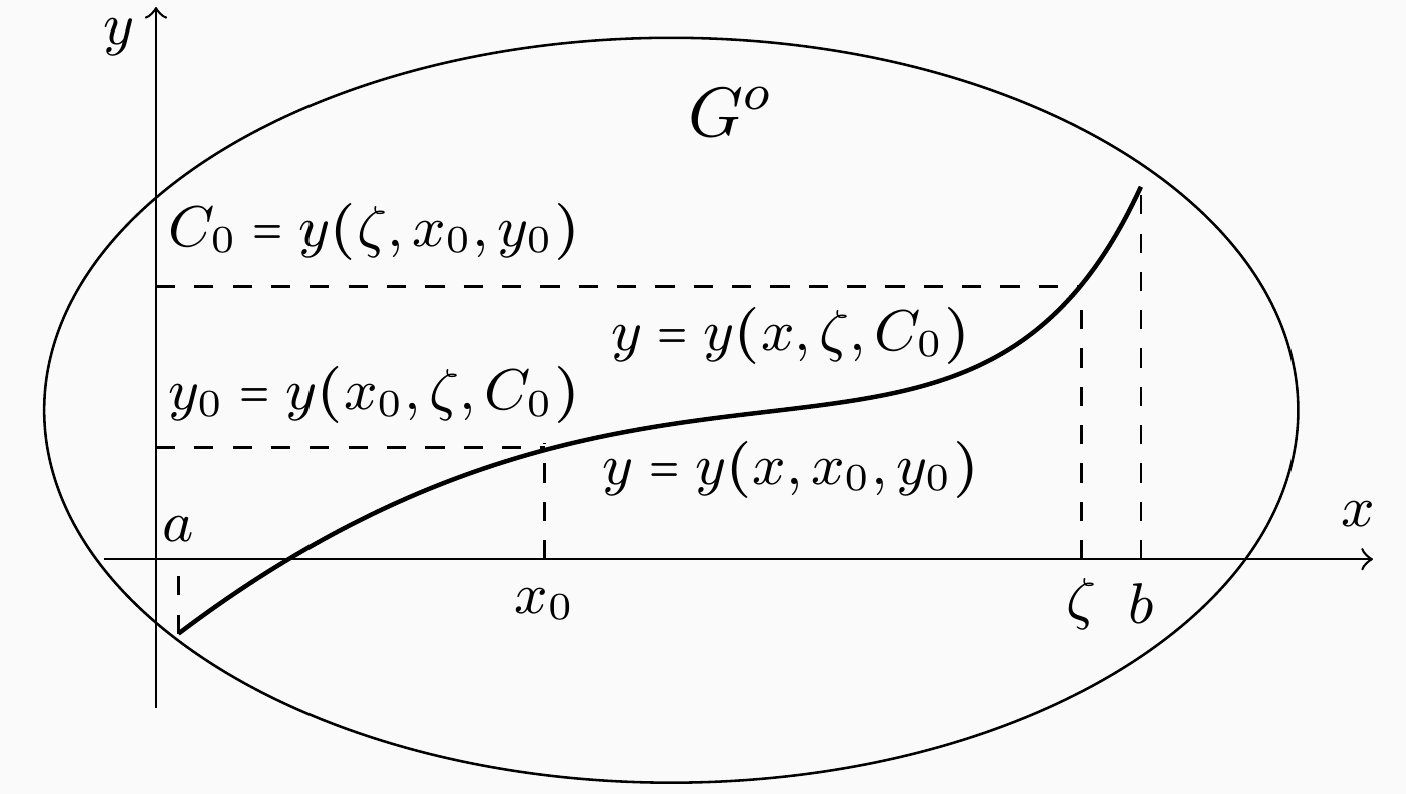
\includegraphics[width=\textwidth]{general_solution}
    \end{subcaptionblock}
    \begin{subcaptionblock}{0.495\textwidth}
    	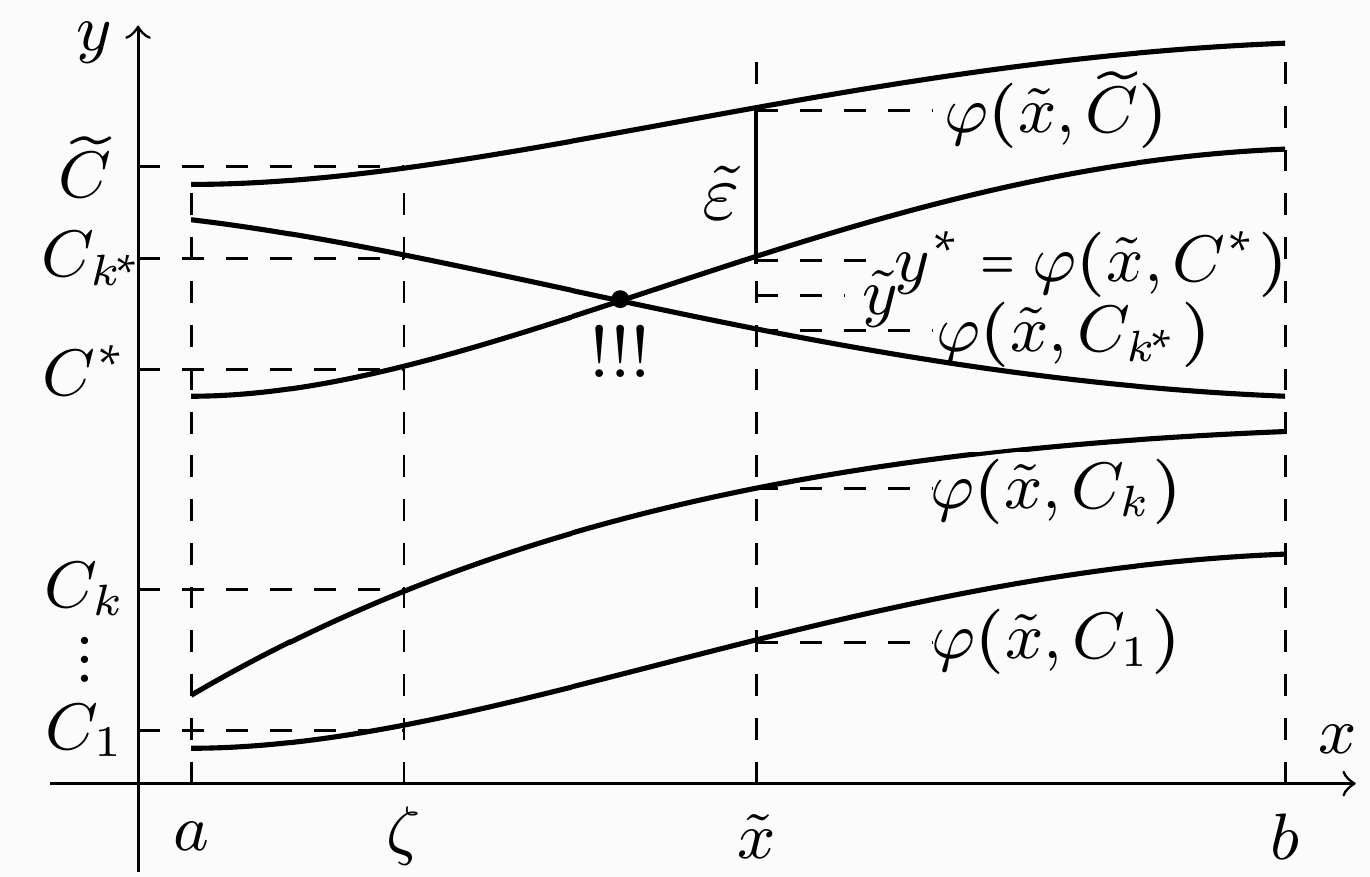
\includegraphics[width=\textwidth]{general_solution_2}
    \end{subcaptionblock}
\end{figure}

\begin{definition}
    Общее решение $ y = \vphi(x, C) $, определённое формулой \eref{1.26}, будем называть общим решением в форме Коши или классическим общим решением уравнения первого порядка \eref{1.1}
\end{definition}

\begin{theorem}[о дифференцируемости общего решения]
    Пусть на компакте $ \ol{A} $ из \eref{1.25} при некотором $ \zeta \in [a, b] $ формула \eref{1.26} задаёт общее решение $ y = \vphi(x, C) $, и в уравнении \eref{1.1} $ f(x, y) $ непрерывно дифференцируема по $ y $ в некоторой окрестности $ \ol{A} $
    \begin{equ}{1.28}
        \implies \quad \forall (x, C) \in \ol{Q} : \quad \pder{\vphi(x, C)}x = \exp \bigg( \dint[t]\zeta{x}{\pder{f \big( t, \vphi(t, C) \big) }y} \bigg)
    \end{equ}
\end{theorem}

\begin{proof}
	Зафиксируем произвольным образом константу $ C \in [\vphi_1(\zeta), \vphi_2(\zeta)] $, после чего для всякого $ x \in [a, b] $ положим $ \Delta \vphi = \vphi(x, C + \Delta C) - \vphi(x, C) $, где $ \Delta C $ -- приращение аргумента $ C $ \\
    Поскольку при фиксированной $ C $ функция $ y = \vphi(x, C) $ является решением уравнения \eref{1.1}, справедлива цепочка равенств:
    \begin{multline*}
        \frac{\di(\Delta \vphi)}{\di x} = f \bigg( x, \vphi(x, C + \Delta C) \bigg) - f \bigg( x, \vphi(x, C) \bigg) = \dint[\bigg( f \big( x, \vphi(x, ) + \Delta \vphi \cdot s \big) \bigg)]01{} = \\
        = \dint[s]01{\frac{\di f \bigg( x, \vphi(x, C) + \Delta \vphi \cdot s \bigg)}{\di s}} = p(x, \Delta C) \Delta \vphi, \qquad p(x, \Delta C) \define \dint[s]01{\pder{f \bigg( x, \vphi(x, C) + \Delta \vphi \cdot s)}y}
    \end{multline*}
    \begin{itemize}
        \item Пусть $ \Delta C \ne 0 $, тогда, поделив первое и последнее выражение в цепочке на $ \Delta C $, убеждаемся, что функция $ \psi(x, \Delta C) \define \dfrac{\Delta \vphi}{\Delta C} $ является решением \caupr{\zeta, 1} линейного однородного уравнения $ \frac{\di u}{\di x} = p(x, \Delta C)u $, так как
        $$ \psi(\zeta, \Delta C) = \frac{\vphi(\zeta, C + \Delta C) - \vphi(\zeta, C)}{\Delta C} \undereq{\eref{1.26}} \frac{C + \Delta C - C}{\Delta C} = 1 $$
        Следовательно, $ \psi(x, \Delta C) = \exp \bigg( \dint[t]\zeta{x}{p(t, \Delta C)} \bigg) $
        \item Но $ p(x, \Delta C) $ существует и при $ \Delta C = 0 $:
        $$ p(x, 0) = \pder{f \bigg( x, \vphi(x, C) \bigg)}y $$
    \end{itemize}
    Поэтому
    $$ \pder{\vphi(x, C)}C = \limz{\Delta C} \psi(x, \Delta C) = \exp \bigg( \limz{\Delta C} \dint[t]\zeta{x}{p(t, \Delta C)} \bigg) $$
    В результате частная производная общего решения $ y = \vphi(x, C) $ по $ C $ существует, непрерывна и вычисляется по формуле \eref{1.28}
\end{proof}

\begin{remark}
    В теореме доказано, что если в уравнении \eref{1.1} правая часть непрерывно дифференцируема по $ y $, то решение $ y = y(x, x_0, y_0) $, рассматриваемое как функция трёх переменных, имеет непрерывную положительнею производную по $ y_0 $
\end{remark}

\chapter{Уравнения первого порядка в симметричной форме}

\section{Существование и единственность решения}

\subsection{Объект изучения}

Уравнение первого порядка в симметрической форме имеет вид
\begin{equ}{2.1}
	M(x, y)\di x + N(x, y) \di y = 0
\end{equ}

и в нём вещественные функции $ M $ и $ N $ определены и непрерывны на связном множестве $ \vawe{B} = B \cup \hat{B} \cup \breve{B} $, где $ B $ -- это область в $ \R^2 $, в которой
\begin{equ}{2.2}
    M^2(x, y) + N^2(x, y) \ne 0
\end{equ}
а множества $ \hat{B}, \breve{B} $, возможно пустые, состоят из граничных точек области $ B $, причём для точек из множества $ \hat{B} $ условие \eref{2.2} выполняется, а лдя точек из множества $ \breve{B} $ -- нет \\
Таким образом, ни в одной из точек множеств $ B $ и $ \hat{B} $ функции $ M $ и $ N $ могут одновременно обратиться в нуль, а для любой точки $ (x, y) \in \breve{B} $ справедливы равенства $ M(x ,y) = N(x ,y) = 0 $ \\
Кроме того, в каждой точке граничного множества $ B^* = \partial B \setminus (\hat{B} \cup \breve{B}) $ хотя бы одна из функций $ M $ или $ N $ не определена или разрывна

\begin{definition}
    Точки из множества $ \breve{B} $ будем называть особыми, а точки из множества $ B \cup \hat{B} $ -- обыкновенными или неособенными
\end{definition}

Уравнение \eref{2.2} будет рассматриваться и решаться на множестве обыкновенных точек, поскольку в особых точках оно фактически вырождается

\subsection{Решение уравнения в симметричной форме}
\label{ssec:simm_solution}

Выделим замкнутые множества нулей функций $ M $ и $ N $:
$$ \ol{M^0} \define \set{(x ,y) \in \vawe{B} | M(x, y) = 0}, \qquad \ol{N^0} \define \set{(x, y) \in \vawe{B} | N(x ,y) = 0} $$
Обозначим через $ \vawe{B_N} $ и $ \vawe{B_M} $ произвольные компоненты связности соответсвенно множества $ \dfrac{\vawe{B}}{\ol{N^0}} $, на котором $ N(x ,y) \ne 0 $ и множества $ \dfrac{\vawe{B}}{\ol{M^0}} $, на котором $ M(x ,y) \ne 0 $. Введём также множество $ \vawe{B}_{MN} = \vawe{B}_M \cap \vawe{B}_N $ \\
Очевидно, что все три разновидности введённых множеств могут иметь общие границы и состоят из обыкновенных точек \\
Уравнение \eref{2.1} на любом из множеств $ \vawe{B}_N $ равносильно уравнению, разрешённому относительно производной
\begin{equ}{2.3_1}
    \frac{\di y}{\di x} = -\frac{M(x, y)}{N(x, y)}
\end{equ}
на множествах $ \vawe{B}_M $ оно равносильно еревёрнутому уравнению
\begin{equ}{2.3_2}
    \frac{\di x}{\di y} = - \frac{N(x, y)}{M(x, y)}
\end{equ}
а на любом из множеств $ \vawe{B}_{MN} $ уравнение в симметричной форме \eref{2.1} равносильно каждому из уравнений \eref{2.3_1}, \eref{2.3_2} \\
Но на любом пожмножестве множества $ \vawe{B}_N $, содержащем хотя бы одну точку из $ \ol{M^0} $, можно перейти только к уравнению \eref{2.3_1}. Аналогично обстоит дело в случае, когда $ \vawe{B}_M \cap \ol{N^0} \ne \O $ \\
Это приводит к вынужденному обобщению понятия решения:

\begin{definition}
    Решением уравнения \eref{2.1} называется определённая на некотром промежутке $ \braket{a, b} $ функция $ y = \vphi(x) $ или функция $ x = \psi(y) $, удовлетворяющая следующим условиям:
    \begin{enumerate}
        \item функция $ \vphi(x) $ или $ \psi(y) $ дифференцируема на $ \braket{a ,b} $
        \item точка $ \big( x, \vphi(x) \big) \in \vawe{B} \setminus \breve{B} $ для любого $ x \in \braket{a, b} $ или \\
        точка $ \big( \psi(y), y \big) \in \vawe{B} \setminus \breve{B} $ для любого $ y \in \braket{a, b} $
        \item $ M \big( x, \vphi(x) \big) + N \big( x, \vphi(x) \big) \vphi'(x) \equiv 0 $ на $ \braket{a, b} $ или \\
        $ M \big( \psi(y), y \big)\psi'(y) + N \big( \psi(y), y \big) \equiv 0 $ на $ \braket{a, b} $
    \end{enumerate}
    При этом решения уравнения \eref{2.1} подразделяются на внутренние, граничные и смешанные в соответствии с аналогичным подразделением решений уравнения \eref{1.1}
\end{definition}

\begin{remark}
	По определению график любого решения состоит только из обыкновенных точек
\end{remark}

\begin{remark}
    По аналогии с уравнением \eref{1.1} для уравнения \eref{2.1} вводится понятие полного решения, в котором максимальный интервал указывается либо для решения $ y = \vphi(x) $, график которого лежит в $ \vawe{B}_N $, любо для решения $ x = \psi(y) $ с графиком из $ \vawe{B}_M $
\end{remark}


\begin{definition}
    Точка $ (x_0, y_0) \in \vawe{B} \setminus \breve{B} $ называется точкой неединственности уравнения \eref{2.1}, если хотя бы для одного из уравнений \eref{2.3_1}, \eref{2.3_2} она окажется точкой неединственности. В противном случае точка $ (x_0, y_0) $ -- это точка единственности
\end{definition}

\begin{remark}
    Решения уравнения \eref{2.1} могут быть частными или особыми точкно так же, как это происходит с решениями уравнения, разрешённого относительно производной
\end{remark}

\subsection{Интегральные кривые}

Уравнение в симметричной форме позволяет обобщить понятие интегральной кривой. Действительно, через каждую точку мноежства $ \vawe{B} \setminus \breve{B} $, используя одно из разрешённых уравнений, можно провести отрезок поля, построив, тем самым, поле направлений уравнения \eref{2.1} \\
Наличие поля направлений позволяет сохранить геометрическое определение интегральной кривой, а именно

\begin{definition}
    Интегральной кривой уравнения \eref{2.1} на множестве $ \vawe{B} \setminus \breve{B} $ назовём любую гладкую кривую, лежащую в этом множестве, напраление касательной к которой в каждой точке совпадает с направлением поля в этой точке
\end{definition}

В результате локально интегральная кривая задаётся или функцией $ y = \vphi(x) $, или $ x = \psi(y) $

\subsection{Существование и единственность решения}

Поскольку уравнение \eref{2.1} в некоторой окрестности любой неособой точки сводится к одному из разрешённых уравнений, то все локальные определения и теоремы из главы 1 остаются верными

\begin{remark}
    В дальнейшем уравнение \eref{2.1} юудет рассматриваться только в области $ B $, в которой по определению рассматриваются только особые точки \\
    В результате по определению все решения будут внутренними и их максимальные интервалы существования всегда будут интервалами
\end{remark}

\begin{theorem}[о существовании решения]
    Пусть в уравнении \eref{2.1} функции $ M(x, y) $ и $ N(x, y) $ непрерывны в области $ B $ \\
    Тогда для любой точки $ (x_0, y_0) \in B $ и для любого отрезка Пеано $ P_h(x_0, y_0) $, построенного для одного из уравнений \eref{2.3_1}, \eref{2.3_2}, определённого в некоторой окрестности $ B_c(x_0, y_0) \sub B $, существует по крайней мере одно решение \caupr[\eref{2.1}]{x_0, y_0}, заданное на $ P_h(x_0 y_0) $
\end{theorem}

\begin{theorem}[о единственности в области; слабая]
    Пусть в уравнении \eref{2.1} функции $ M(x, y) $ и $ N(x, y) $ непрерывны в области $ B $, а в области $ B^0 \sub B $ верно хотя бы одно из двух условий:
    \begin{itemize}
    	\item $ N(x, y) \ne 0, \quad $ существуют и непрерывны частные производные $ M_y'(x, y) $, $ N_y'(x, y) $
        \item $ M(x, y) \ne 0, \quad $ существуют и непрерывны чатсные производные $ M_x'(x, y), N_x'(x, y) $
    \end{itemize}
    Тогда $ B^0 $ -- это область единственности
\end{theorem}

\begin{proof}
    Действительно, при выполнении первого условия, например, в области $ B^0 $ уравнение \eref{2.1} равносильно уравнению \eref{1.1} с $ F = -\frac{M(x, y)}{N(x, y)} $, и частная производная $ \pder{f}y = \dfrac{M \pder{N}y - N \pder{M}y}{N^2} $ непрерывна, а значит, верна слабая теорема о единственности (теор. \ref{th:uniq:weak})
\end{proof}

\begin{implication}
	Область $ B $ будет областью единственности, если найдётся открытое покрытие её областями, для каждой их которых выполняется хотя бы одно из приведённых в формулировке теоремы условий
\end{implication}

\section{Интергал уравнения в симметричной форме}

\subsection{Определение интеграла}

Интегральные кривые уравнения в симметричной форме по определению могут иметь любые касательные. Параметризуют их непрерывные неявные функции $ U(x, y) = 0 $. Именно в таком виде будем искать решение уравнения \eref{2.1}, называя их при этом интегралами. Аналог общего решения будем называть общим интегралом

\begin{definition}
	Непрерывную в области $ B \sub \R^2 $ функцию $ U(x, y) $ будем называть допустимой, если для любой точки $ (x_0, y_0) \in B $ найдётся такая непрерывная функция $ y = \xi(x) $ или $ x = \eta(y) $, определённая на интервале $ (\alpha, \beta) $, содержащем точку $ x_0 $ или $ y_0 $, что:
    \begin{enumerate}
    	\item $ y_0 = \xi(x_0) $ или $ x_0 = \eta(y_0) $
        \item точка $ \big( x, \xi(x) \big) \in B $ для любого $ x \in (\alpha, \beta) $ или \\
        точка $ \big( \eta(y), y \big) \in B $ для любого $ y \in (\alpha, \beta) $
        \item $ y = \xi(x) $ или $ x = \eta(y) $ -- единственное решение уравнения
        \begin{equ}{2.6}
        	U(x, y) = U(x_0, y_0)
        \end{equ}
    \end{enumerate}
\end{definition}

\begin{remark}
	Условие 3 означает, что выполняется по крайней мере одно из тождеств:
    $$
    \begin{vars}
        U \big( x, \xi(x) \big) \overset{(\alpha, \beta)}\equiv U(x_0, y_0) \\
        U \big( \eta(y), y \big) \overset{(\alpha, \beta)}\equiv U(x_0, y_0)
    \end{vars} $$
\end{remark}

В дальнейшем будем всегда предполагать, что $ B $ -- это область единственности, так как общий интеграл может быть построен только в области единственности

\begin{definition}
    Допустимая функция $ U(x, y) $ назыается интегралом уравнения \eref{2.1} в области единственности $ B^0 $, если для любой точки $ (x_0, y_0) \in B^0 $ единственная функция $ y = \xi(x) $ или $ x = \eta(y) $ из определения допустимой функции -- это решение \caupr[\eref{2.1}]{x_0, y_0} на $ (\alpha, \beta) $, т. е. удовлетворяет тождеству $ 3_1 $ или $ 3_2 $ из определения решения
\end{definition}

\subsection{Характеристической свойство интеграла}

\begin{note}
	В математике часто характеристическим свойством назвыают другое определение того же объекта
\end{note}

\begin{theorem}[о характеристическом свойстве интеграла]
    Для того чтобы допустимая функция $ U(x, y) $ была интегралом уравнения в симметричной форме \eref{2.1} в области единственности $ B^0 $, \bt{необходимо и достаточно}, чтобы $ U(x, y) $ обращалась в постоянную вдоль любого решения \eref{2.1}, т. е. чтобы:
    \begin{itemize}
        \item $ U \big( x, \vphi(x) \big) \overset{\braket{a, b}}\equiv C $ для любого решения $ y = \vphi(x) $, определённого на $ \braket{a, b} $
        \item $ U \big( \psi(y), y \big) \overset{\braket{a, b}}\equiv C $ для любого решения $ x = \vphi(y) $, определённого на $ \braket{a, b} $
    \end{itemize}
\end{theorem}

\begin{iproof}
	\item Необходимость: \\
    Пусть $ U(x, y) $ -- интеграл уравнения \eref{2.1} в области единственности $ B^0 $, и пусть, например, $ y = \vphi(x) $ -- какое-либо решение уравнения \eref{2.1}, определённое на промежутке $ \braket{a, b} $ \\
    НУО\footnotemark будем считать, что $ \braket{a, b} = (a, b) $ \\
    Возьмём произвольную точку $ x_0 \in (a, b) $ и положим $ y_0 \define \vphi(x_0) $ \\
    Точка $ (x_0, y_0) \in B^0 $, поэтому по определению допустимой функции уравнение \eref{2.6} $ U(x, y) = U(x_0, y_0) $ однозначно разрешимо или относительно $ x $, или относительно $ y $:
    \begin{itemize}
        \item Пусть \eref{2.6} однозначно разрешимо относительно $ y $, т. е. существует такая единственная функция $ y = \xi(x) $, заданная на некотором $ (\alpha, \beta) \ni x_0 $, что $ U \big( x, \xi(x) \big) \overset{(\alpha, \beta)}\equiv U(x_0, y_0) $ \\
        Эта функция по опреелению интеграла является решением \caupr[\eref{2.1}]{x_0, y_0} \\
        Поскольку $ B^0 $ -- область единственности, $ \vphi(x) \overset{(\vawe\alpha, \vawe\beta)}\equiv \xi(x) $, где $ (\vawe\alpha, \vawe\beta) = (a, b) \cap (\alpha, \beta) $. Следовательно,
        \begin{equ}{2.7}
            U \big( x, \vphi(x) \big) \overset{(\vawe\alpha, \vawe\beta)}\equiv U(x_0, y_0)
        \end{equ}
        \item Пусть \eref{2.6} однозначно разрешимо относительно $ x $, т. е. на некотором интервале $ (\alpha, \beta) \ni y_0 $ существует единственная функция $ x = \eta(y) $ такая, что $ \eta(y_0) = x_0 $ и $ U \big( \eta(y), y \big) \equiv U(x_0, y_0) $ на $ (\alpha, \beta) $ \\
        Тогда по определению интеграла $ x = \eta(y) $ на $ (\alpha, \beta) $ является решением \caupr[\eref{2.1}]{y_0, x_0}, а значит, единственное решение этой ЗК имеет два представления: $ y = \vphi(x) $ и $ x = \eta(y) $. Поэтому дуга интегральной кривой такого решения в некоторой окрестности точки $ (x_0, y_0) $, не имея вертикальных и горизонтальных касательных, может быть параметризована как функцией $ y = \vphi(x) $, так и функцией $ x = \eta(x) $ \\
        Иными словами, сущетвуют такие интервалы $ (\vawe{a}, \vawe{b}) $ и $ (\vawe\alpha, \vawe\beta) $, что
        $$ x_0 \in (\vawe{a}, \vawe{b}) \sub (a, b), \quad y_0 \in (\vawe\alpha, \vawe\beta) \sub (\alpha, \beta), \qquad y \overset{(\vawe\alpha, \vawe\beta)}\equiv \vphi \big( \eta(y) \big), \quad x \overset{(\vawe{a}, \vawe{b})}\equiv \eta \big( \vphi(x) \big) $$
        Поэтому справедлива доказывающая \eref{2.7} цепочка равенств:
        $$ U \big( x, \vphi(x) \big) \overset{)\vawe{a}, \vawe{b}}\equiv U \bigg( \eta \big( \vphi(x) \big), \vphi(x) \bigg) \overset{(\vawe\alpha, \vawe\beta)}\equiv U \big( \eta(y), y \big) \overset{(\vawe\alpha, \vawe\beta)}\equiv U(x_0, y_0) $$
        \item Осталось показать, что \eref{2.7} выполняется на всём интервале $ (a, b) $: \\
        \bt{Допустим}, что $ \vawe\beta < b $ и найдутся такие $ x_1, x_2 \in [\vawe\beta, b) $, ($ x_1 < x_2 $), что $ U \big( x, \vphi(x) \big) \overset{(\vawe\alpha, x_1]}\equiv U(x_0, y_0), \quad U \big( x, \vphi(x) \big) \neq U(x_0, y_0) $ для любого $ x \in (x_1, x_2) $ \\
        При $ y_1 = \vphi(x_1) $ в последнем тождестве $ U(x_1, y_1) = U(x_0, y_0) $. По определению решения точка $ (x_1, y_1) \in B^0 $, поэтому для неё верны все рассуждения, касающщиеся точки $ (x_0, y_0) $ \\
        Пусть $ y = \xi_1(x) $ -- единственное на $ (\alpha_1, \beta_1), \quad \bigg( x_! \in (\alpha_1, \beta_1) \sub (x_0, x_2) \bigg) $ решение уравнения $ U(x, y) = U(x_1, y_1) $, т. е. $ U \big( x, \xi_1(x) \big) \equiv U(x_1, y_1) $ на $ (\alpha_1, \beta_1) $, и оно же по определению интеграла является единственным решением \caupr{x_1, y_1}. Тогда $ \xi_1(x) \equiv \vphi(x) $ на $ (\alpha_1, \beta_1) $, и $ U \big( x, \vphi(x) \big) \overset{[x_1, \beta_1)}\equiv U(x_1, y_1) = U(x_0, y_0) $ -- \contra \\
        Ситуация с точками $ x_1, x_2 \in (a, \vawe\alpha] $ рассматривается аналогично
        \item Достаточность: \\
        Пусть допустимая функция $ U(x, y) $ обращается в постоянную на любом решении уравнения \eref{2.1}. Покажем, что в таком случае $ U(x, y) $ -- интеграл этого уравнения в области едиснтвенности $ B^0 $ \\
        Возьмём произвольную точку $ (x_0, y_0) \in B^0 $. Тогда существует единственное решение \\ \caupr{x_0, y_0} вида $ y = \vphi(x) $ на $ (a ,b) \ni x_0 $, или $ x = \psi(y) $ на $ (a, b) \ni y_0 $ \\
        Пусть, например, $ x = \psi(y) $ является решением уравнения \eref{2.1}. Тогда по условию теоремы $ U \big( \psi(y), y \big) \equiv U(x_0, y_0) $ на $ (a, b) $ \\
        Если функция $ U(x, y) $, будучи допустимой, однозначно разрешима относительно $ x $, т. е. на некотором $ (\alpha, \beta) \ni y_0 $ существует и единственна функция $ x = \eta(y) $ такая, что $ U \big( \eta(y), y \big) \equiv U(x_0, y_0) $ на $ (\alpha, \beta) $, то $ \psi(y) \equiv \eta(y) $ на $ (a, b) \cap (\alpha, \beta) $. А если уравнение \eref{2.6} однозначно разрешимо относительно $ y $, то можно показать, как и при доказательстве необходимости, что функция $ y = \xi(x) $ -- решение уравнения \eref{2.1}, поскольку является обратной к решению $ x = \psi(y) $ \\
        В результате допустимая функция $ U(x, y) $ -- это интеграл уравнения \eref{2.1} в области единственности $ B^0 $
    \end{itemize}
    \footnotetext{Действительно, если $ \braket{a, b} = [a, b] $, то по лемме о продолжимости решения, решение может быть продолжено на интервал $ (a_1, b_1) \supset [a, b] $}
\end{iproof}

\subsection{Характеристическое свойство гладкого интеграла}

\begin{definition}
	Гладкую функцию $ U(x, y) $ будем называть галдкой допустимой в области $ B $, если $ U_x'^2 + U_y'^2 > 0 $ для любой точки $ (x, y) \in B $
\end{definition}

\begin{definition}
    Интеграл $ U(x, y) $ уравнения \eref{2.1} будем называть гладким, если $ U $ -- гладкая допустимая функция
\end{definition}

\begin{theorem}[о характеристическом свойстве гладкого интеграла]
    Для того чтобы гладкая допустимая функция $ U(x, y) $ была гладким интегралом уравнения \eref{2.1} в области единственности $ B^0 $, \bt{необходимо и достаточно}, чтобы выполнялось тождество
    \begin{equ}{2.8}
        N(x, y) U_x'(x, y) - M(x, y)U_y'(x,y) \overset{B^0}\equiv 0
    \end{equ}
\end{theorem}

\begin{iproof}
    \item Необходимость \\
    Пусть $ U(x, y) $ -- это гладкий интеграл уравнения \eref{2.1}. Возьём любую точку $ (x_0, y_0) \in B^0 $ \\
    Тогда $ M^2(x_0, y_0) + N^2(x_0, y_0) \ne 0 $. Пусть, например, $ N(x_0, y_0) \ne 0 $ \\
    Тогда $ (x_0, y_0) \in B_N^0 $, где $ B_N^0 $ -- некая компонента связности открытого множества $ B^0 \setminus \ol{N}_0 $ (см. п. \ref{ssec:simm_solution}), в которой $ N(x, y) \ne 0 $ и уравнение \eref{2.1} равносильно уравнению \eref{2.3_1} \\
    Пусть $ y = \vphi(x) $ -- решение \caupr[\eref{2.1}, \eref{2.3_1}]{x_0, y_0}, определённое на некотором интервале $ (a, b) \ni x_0 $ \\
    Тогда по определению решениия
    $$ \vphi'(x) \equiv -\frac{M \big( x, \vphi(x) \big)}{N \big( x, \vphi(x) \big)} \quad \text{ на } (a, b) $$
    По теореме о характеристическом свойстве интегала имеем:
    $$ U \big( x, \vphi(x) \big) \overset{(a, b)}\equiv U(x_0, y_0) $$
    Продиффиренцируем по $ x $:
    $$ U_x' \big( x, \vphi(x) \big) + U_y' \big( x, \vphi(x) \big) \vphi'(x) \overset{(a, b)}\equiv 0 $$
    Подставляя $ \vphi'(x) $ и домножая на $ N $, получаем:
    $$ N \big( x, \vphi(x) \big)U_x' \big( x, \vphi(x) \big) - M \big( x, \vphi(x) \big)U_y' \big( x, \vphi(x) \big) \overset{(a, b)}\equiv 0 $$
    Положим $ x = x_0 $, тогда $ \vphi(x_0) = y_0 $, и для любой точки $ (x_0, y_0) \in B^0 $ получаем равенство \eref{2.8}
    \item Достаточность \\
    Пусть в $ B^0 $ выполняется тождество \eref{2.8} \\
    Возьмём любую точку $ (x_0, y_0) \in B^0 $, и пусть, например, $ U_y'(x_0, y_0) \ne 0 $ \\
    Тогда $ U_y'(x, y) \ne 0 $ в некоторой окрестности $ V(x_0, y_0) $ и в ней уравнение \eref{2.6} $ U(x, y) = U(x_0, y_0) $ однозначно разрешимо относительно $ y $, т. е. существует и единственна функция $ y = \xi(x) $, определённая на нектором интервале $ (\alpha, \beta) \ni x_0 $ такая, что $ \xi(x_0) = y_0, \quad \xi \in \Cont[1]{(\alpha, \beta)} $ и $ U \big( x, \xi(x) \big) \equiv U(x_0, y_0) $ на $ (\alpha, \beta) $ \\
    Дифференцируя последнее тождество, получаем
    $$ U_x' \big( x, \xi(x) \big) + U_y' \big( x, \xi(x) \big) \xi'(x) \overset{(\alpha, \beta)}\equiv 0, \qquad \big( x, \xi(x) \big) \in V $$
    а значит, $ \xi'(x) \equiv -\dfrac{U_x' \big(x, \xi(x) \big)}{U_y' \big( x, \xi(x) \big)} $ \\
    Покажем, что $ y = \xi(x) $ является решением уравнения \eref{2.1}, т. е. на интервале $ (a, b) $, например, удовлетоворяет тождеству $ 3_1 $ из определения решения. Подставляя $ \xi(x) $ в левую часть этого тождества, получаем:
    $$ M \big(x, \xi(x) \big) + N \big(x, \xi(x) \big) \xi'(x) \equiv \frac{M \big(x, \xi(x) \big)U_y' \big( x, \xi(x) \big) - N \big( x, \xi(x) \big)U_x' \big( x, \xi(x) \big)}{U_y' \big( x, \xi(x) \big)} \overset{\eref{2.8}}\equiv 0 $$
\end{iproof}

\begin{implication}
    Гладкая допустимая функция $ U(x, y) $ есть гладкий интеграл уравнения \eref{1.1} $ y' = f(x, y) $ в области единственности $ G^0 $ \bt{тогда и только тогда}, когда верно тождество
    $$ U_x'(x, y) + f(x, y)U_y'(x, y) \overset{G^0}\equiv 0 $$
\end{implication}

\subsection{Существование интеграла, связь между интегралами}

\begin{theorem}[о существовании непрерывнорго ингеграла]
    Для любой точки $ (x_0, y_0) $ из области единственности $ B^0 $ найдётся окрестность $ S \sub B^0 $, в которй уравнение \eref{2.1} имеет интеграл $ U(x, y) $
\end{theorem}

\begin{proof}
    Пусть $ (x_0, y_0) $ "--- это произвольная точка из области едлинственности $ B^0 $ и, например, $ N(x_0, y_0) \ne 0 $. Тогда найдётся окрестность $ B_N^0 $, в которой $ N(x, y) \ne 0 $, а значит, в ней уравнение в симметричной форме \eref{2.1} равносильно уравнению \eref{2.3_1} $ y' = - \frac{M(x, y)}{N(x, y)} $ \\
    Согласно теореме о существовании общего решения в области
    $$ A = \set{(x,y) | a < x < b, \quad \vphi_1(x) < y < \vphi_2(x)} \sub B_N^0 $$
    существует общее решение $ y = \vphi(x, C) $ уравнения \eref{2.3_1} \\
    По определению общего решения уравнение $ y = \vphi(x, C) $ однозанчно разрешимо относительно $ C $ для любой точки $ (x, y) \in A $, т. е. $ C = U(x, y) $, причём $ U \big( x, \vphi(x, C) \big) \overset{(a, b)}\equiv C $ \\
    В результате уравнение $ U(x, y) = C $ однозначно разрешимо относительно $ y $, а значит, функция $ U $ -- допустимая и постоянна вдоль любого решения, график которого лежит в области $ A $ \\
    По теореме о характеристическом свойстве интеграла функция $ U(x, y) $ является интегралом уравнения \eref{2.1} в области $ A $
\end{proof}

\begin{definition}
    $ U(x, y) $ -- интеграл уравнения \eref{2.1} в области единственности $ B^0 $ \\
    Тогда равенство $ U(x, y) = C $ называется общим интегралом уравнения \eref{2.1}
\end{definition}

\begin{theorem}[о существовании гладкого интеграла]
    \hfill \\
    В уравнении \eref{2.1} функции $ M(x, y), ~ N(x, y) \in \Cont[1]B $ \\
    Тогда для любой точки $ (x_0, y_0) $ из области $ B $ существует её окрестность $ A \sub B $, в которой уравнение \eref{2.1} имеет гладкий интеграл $ U(x, y) $
\end{theorem}

\begin{proof}
	По слабюой теореме о единственности в области множество $ B $ является областью единственности \\
    Возьмём любую точку $ (x_0, y_0) $ из $ B $. И пусть, например, $ N(x_0, y_0) \ne 0 $, $ B_N $ "--- окрестность $ (x_0, y_0) $, в которой $ N(x, y) \ne 0 $ и уравнение \eref{2.1} равносильно уравнению \eref{2.3_1} $ y' = f_*(x, y) $ с $ f_* \define - \frac{M(x, y)}{N(x, y)} $. При этом по условию теоремы в области $ B_N $ определена и непрерывна частная производная $ \pder{f_*(x, y)}y $ \\
    Пусть $ A \define \set{(x, y) | a < x < b, \quad \vphi_1(x) < y < \vphi_2(x)} $ "--- окрестность точки $ (x_0, y_0) $, лежащая в $ B_N $ вместе со своим замыканием. По теореме о существовании общего решения в $ A $ существует общее решение $ y = \vphi(x, C) $ уравнения $ y' = f_*(x, y) $, задаваемое формулой \eref{1.26} $ \vphi(x, C) = y(x, \xi C) $, в которой $ \xi \in (a, b) $ выбирается произвольным образом, $ (\xi, C) \in \ol{A} $, т. е. $ C \in [\vphi_1(\xi), \vphi_2(\xi)] $, а $ y(x, \xi, C) $ "--- решение \caupr{\xi, C} \\
    Положим $ \xi = x_0 $. Согласно \eref{1.28}
    $$ \pder{\vphi(x, C)}C = \exp \bigg( \dint[t]{x_0}x{\pder{f_* \big( t, \vphi(t, C) \big)}y} \bigg), \qquad \pder{\vphi(x_0, C)}C = 1 \quad \forall C \in [\vphi_1(x_0), \vphi_2(x_0)] $$
    Следовательно, по теореме о неявной функции уравнение $ \vphi(x, C) - y = 0 $ однозначно разрешимо относительно $ C $. Его решение $ C = U(x, y) $, как установлено в доказательстве теоремы о существовании непрерывного интеграла, является интегралом уравнения \eref{2.1} и непрерывно дифференцируемо по $ y $ в области $ A $
\end{proof}
